\documentclass[11pt,a4paper]{article}
% Journal-agnostic submission draft. Anonymous for review; the title page with author details is
% title_page.tex. Reformat to the target journal's class by replacing this preamble and the
% bibliography style only: all content lives in the \input files.
\usepackage[margin=2.5cm]{geometry}
\usepackage[T1]{fontenc}
\usepackage{lmodern}
\usepackage{microtype}
\usepackage{amsmath,amssymb,amsthm}
\usepackage{booktabs,multirow,array}
\usepackage{graphicx}
\usepackage{xcolor}
\usepackage[numbers,sort&compress]{natbib}
\usepackage{algorithm}
\usepackage{algpseudocode}
\usepackage{hyperref}
\usepackage{setspace}
\onehalfspacing
\hypersetup{colorlinks=true,linkcolor=blue!50!black,citecolor=blue!50!black,urlcolor=blue!50!black}
\renewcommand{\topfraction}{0.95}\renewcommand{\textfraction}{0.05}\renewcommand{\floatpagefraction}{0.8}
\setcounter{topnumber}{4}\setcounter{totalnumber}{6}

\theoremstyle{plain}
\newtheorem{theorem}{Theorem}
\newtheorem{proposition}{Proposition}
\newtheorem{lemma}{Lemma}
\newtheorem{corollary}{Corollary}
\theoremstyle{definition}
\newtheorem{definition}{Definition}
\newtheorem{assumption}{Assumption}
\theoremstyle{remark}
\newtheorem{remark}{Remark}

\newcommand{\Risk}{\mathcal{R}}
\newcommand{\Cov}{\mathcal{C}}
\newcommand{\emit}{\mathcal{E}}
\newcommand{\E}{\mathbb{E}}
\renewcommand{\Pr}{\mathbb{P}}
\newcommand{\Iota}{\mathcal{I}}
\newcommand{\ind}[1]{\mathbf{1}\{#1\}}

\title{Certified Correction of Vision--Language Hallucinations:\\
Guarantees, Gains and Failure Modes under a Pre-specified Protocol}
\author{Anonymous Author(s)}
\date{}

\begin{document}
\maketitle

\begin{abstract}
Selective prediction gives a vision--language model (VLM) a distribution-free guarantee on the
answers it emits and pays for it by abstaining on the rest. When the base error rate $\mu$
exceeds the target $\alpha$, any predictor that may only emit or abstain the model's own answer
must abstain on at least $(\mu-\alpha)/(1-\alpha)$ of inputs. We ask what changes when the
predictor may emit a different answer. Certified-Correction Risk Control (CCRC) accepts the
model's answer where a correctness score is high, substitutes the answer of a distinct evidence
source (here an open-vocabulary detector) where that source is decisive, abstains otherwise, and
certifies the error rate of everything emitted with a fixed-sequence Clopper--Pearson test.

We prove validity for policy families indexed by pre-specified score values under i.i.d.
sampling of calibration units, and we evaluate CCRC under a protocol built so that the proved
procedure and the evaluated procedure coincide: folds are unions of whole images, thresholds and
repair gate are values fixed before calibration, the start of the test sequence is derived
analytically, and the repair gate is fixed on external data, chosen on the fit fold, or
certified by a union bound. On five benchmark--backbone cells, certified coverage over
filtering changes by $+0.8$ to $+7.9$ points with an externally fixed gate, positive in all ten
(cell, $\alpha$) combinations; an outer image-level bootstrap excludes zero only on the largest
cell (250 images). Most of the repaired mass re-emits the model's own answer with detector
confirmation, and only $0.04$--$1.7\%$ of test items have their answer changed; no
false-positive existence error is corrected. The correctness score, not the repair, supplies
most of the coverage, and fixed-sequence testing started at the minimal certifiable emitted set
is fragile with small calibration folds. A matched-prefix experiment shows that mid-caption repair
increases downstream hallucination, which blocks a fixed-point route to a sequential guarantee.
\end{abstract}

\section{Introduction}
\label{sec:intro}

A vision--language model that answers ``is there a mouse in the image?'' wrongly is more
useful if it says so. Selective prediction does this: a score ranks the model's answers, a
threshold is calibrated on held-out data, and the model answers only above it. Conformal and
risk-controlling variants \citep{bates2021rcps,angelopoulos2021ltt,angelopoulos2024crc} certify,
with a finite-sample guarantee that makes no assumption on the score or the model, that the
error rate among the answers that are emitted stays below a target $\alpha$.

The guarantee is paid for in coverage, and part of the bill cannot be reduced. Kotte
\citep{crcimposs} shows that when the base error rate $\mu$ exceeds $\alpha$, any predictor that
may only emit or abstain the model's own answer must abstain on at least
$(\mu-\alpha)/(1-\alpha)$ of inputs, whatever the score, the concentration inequality or the
calibration budget (Proposition~\ref{prop:floor} below). The proof uses one premise: an
abstained item is an item whose model answer stays wrong. A predictor that may emit a
\emph{different} answer is outside the premise.

This paper studies that possibility in the simplest setting where it can be made exact: yes/no
object-existence questions, with an open-vocabulary detector as a second, distinct source of
evidence. \emph{Certified-Correction Risk Control} (CCRC) accepts the model's answer where a
correctness score is high, replaces it with the detector's answer where the detector's evidence
is decisive, abstains otherwise, and certifies the error rate of the whole emitted set, accepted
and substituted answers together.

\paragraph{What the paper contributes.}
Our aim is a result that survives a strict reading of the protocol. Four design decisions follow
from that aim, and each is a contribution in its own right.
\begin{enumerate}
\item \emph{The proved procedure is the evaluated procedure.} Theorem~\ref{thm:validity} covers
  policy families indexed by threshold \emph{values} fixed before calibration under i.i.d.
  sampling of calibration units. Every reported number uses such a family: thresholds and repair
  gate are read off the fit fold, never off the calibration sample whose errors are counted.
\item \emph{The sampling unit is stated and respected.} POPE contributes six questions per
  image; folds here are unions of whole images, we measure the within-image dependence of
  errors, and a known-population simulation shows how clustering would degrade the guarantee and
  how a one-item-per-image calibration restores it.
\item \emph{The repair gate is not tuned on the evaluation data.} We report three ways of
  fixing it that keep the guarantee: a constant chosen on a different benchmark, a choice made
  on the fit fold, and a union bound over a pre-specified set of gates.
\item \emph{Uncertainty is stated at the level of the data.} Gains are accompanied by an outer
  image-level bootstrap, because hundreds of random splits of one benchmark measure the
  procedure's sensitivity to the split, not the benchmark's sampling error.
\end{enumerate}

\paragraph{What we find.}
\begin{itemize}
\item With the gate fixed on an external benchmark, CCRC certifies $+0.8$ to $+7.9$ points more
  coverage than filtering in all ten (cell, $\alpha$) combinations, and the image-bootstrap
  interval excludes zero only on the largest cell (250 images). On the others the sign is
  right in $65$--$95\%$ of bootstrap replicates but cannot be called (\S\ref{sec:main}).
\item Choosing the gate on the fit fold, or certifying three gates by a union bound, is valid
  but costs more than it returns when the calibration fold holds $150$--$200$ items
  ($-6.2$ to $+9.4$ and $-16.5$ to $+4.4$ points over all cells); with $500$ items both help.
\item The repair is mostly confirmation. Between $41$ and $96\%$ of repaired items are items on
  which the detector agrees with the model, and the answer is changed for only $0.04$--$1.7\%$
  of test items. The one-directional gate never corrects a false-positive existence error, and
  a polarity-symmetric gate does not either (\S\ref{sec:accounting}).
\item The start of the fixed sequence matters more than the repair on small folds. Starting
  where a single error can be tolerated ($k\ge38$ at $\alpha=\delta=0.10$) rather than where
  none can ($k\ge22$) raises filtering coverage on the smallest cell (calibration folds of $150$ items) from $22\%$
  to $41\%$ when the first hypothesis sits at the minimal count, and removes the apparent loss on
  AMBER that the conventional start produces (\S\ref{sec:start}).
\item Certified coverage comes mostly from the score: a detection-grounded score certifies
  $68\%$ on POPE-1500 against $41\%$ for model confidence and $0.5\%$ for the image--text
  similarity score of ConfLVLM, while certified repair adds $3$--$6$ points
  (\S\ref{sec:score}).
\item In free-form generation, repairing a claim mid-caption increases downstream
  hallucination in a matched-prefix experiment (\S\ref{sec:sequential}), which blocks the
  fixed-point argument we had hoped to use for a sequential guarantee.
\end{itemize}

\paragraph{Scope.}
Everything here concerns binary existence questions, one detector, one family of backbones and
benchmarks whose images overlap ($642$ distinct images across all cells, and the POPE-adversarial
cells are subsets of the POPE-1500 cell's $250$ images). We do not claim that correction is
generally useful, only that under a protocol whose guarantee we can state it is valid and its
gain is measured.

\section{Related work}
\label{sec:related}

The survey covers work available up to 4 October 2026; claims of the form ``no method does X'' refer
to the literature we surveyed up to that date and are not claims about the field.

\paragraph{Hallucination in vision--language models.}
Multimodal hallucination is usually split into existence, attribute and relation errors
\citep{amber}; surveys \citep{bai2024survey,liu2024survey,ji2023} attribute it to language-prior
dominance, weak visual attention, instruction-tuning artefacts \citep{liu2023lrv} and
miscalibration \citep{guo2017}. Existence claims can be checked by an open-vocabulary detector
\citep{owlv2,liu2024groundingdino}; attribute and relation claims need finer perception than a
detector supplies, which is why the benchmark's composition, and not only its difficulty,
determines whether our evidence channel applies (\S\ref{sec:noevidence}). POPE \citep{pope}
probes existence with balanced yes/no questions under random, popular and adversarial negative
sampling; AMBER \citep{amber} adds an LLM-free discriminative split; MME \citep{mme}, GQA
\citep{gqa} and HallusionBench \citep{hallusionbench} are used here as settings where the detector
mostly does not apply.

Mitigation methods modify decoding \citep{opera,vcd,chen2024halc,favero2024,degf,marine},
intervene on heads or positional structure \citep{attnlens,only,maskcd,causalgating,mcallava},
retrain \citep{sun2024aligning,yu2024rlhfv,liu2023lrv}, or verify and rewrite after generation
\citep{woodpecker,lure,reverse,mkgrag,rule,cmvkgguard}. Post-hoc verification performs the same
three steps as CCRC (flag, consult external evidence, substitute) and none of these systems
certifies the substitution. Lowering the base risk $\mu$ lowers the abstention floor, so these
methods compose with ours; \S\ref{sec:score} runs CCRC on top of visual contrastive decoding.

\paragraph{Conformal prediction and distribution-free risk control.}
Conformal prediction \citep{vovk2005,papadopoulos2002,lei2018,angelopoulos2023gentle} gives
finite-sample coverage under exchangeability. Risk-controlling prediction sets \citep{bates2021rcps}
and conformal risk control \citep{angelopoulos2024crc} control the expectation of a monotone
loss; Learn-then-Test \citep{angelopoulos2021ltt} treats the choice among configurations as
multiple testing and admits fixed-sequence testing over a pre-ordered family at full $\delta$,
which we use. For a binary loss the exact Clopper--Pearson bound \citep{clopper1934} is tighter
than Hoeffding, empirical Bernstein or betting bounds \citep{waudbysmith2024}.
Selective prediction with abstention predates the conformal treatment
\citep{chow1970,elyaniv2010,bartlett2008,cortes2016,geifman2019}; the floor of
Proposition~\ref{prop:floor} concerns the action space and applies to these formulations too.

\paragraph{Conformal methods for language and vision--language models.}
Conformal language modelling \citep{conformallm} calibrates sampling, stopping and rejection;
conformal factuality \citep{conformalfactuality} backs off to a subset of claims;
coherent factuality \citep{rubintoles2025coherent} filters whole reasoning steps; adaptive
variants improve conditional coverage of the filter \citep{rubashevskii2026adaptive}; and a robustness
audit shows that claim filtering for retrieval-augmented models becomes vacuous at high
factuality levels and is fragile to shift \citep{chen2026ragconformal}. Conformal alignment
\citep{gui2024conformal}, conformal multiple choice \citep{kumar2023} and calibrated help-seeking
\citep{ren2023knowno} certify act-or-defer decisions. In the multimodal setting ConfLVLM
\citep{conflvlm} filters unsupported claims scored by image--text similarity, Wagner et al.\
\citep{twoaxes} study abstention along correctness and answerability, and IntroConformal
\citep{atabuzzaman2026introconformal} builds conformity scores from the model's hidden states and
self-verification, without external verifiers. Inference-time conformal reasoning
\citep{wang2026itcr} moves calibration inside generation and intervenes by truncating. All of
these filter, back off, stop or abstain. One method certifies a revised output:
conformal linguistic calibration \citep{jiang2025clc} replaces claims by less specific ones with a
guarantee on the rewritten text; it is text-only and the rewrite generalises a claim rather than
substituting externally verified evidence.

\paragraph{Learning to defer, cascades and routing.}
Emitting the answer of a second predictor is the action of learning to defer, where a policy decides when a decision-maker or expert answers instead of
the model \citep{madras2018defer,mozannar2020defer}; classical rejection learning \citep{cortes2016} abstains at a constant cost. Cascades and
routing send an input to a cheaper or stronger model by confidence \citep{chen2024frugalgpt}, and several recent methods add statistical guarantees:
cascaded selective evaluation certifies agreement with human judgments by fixed-sequence testing over LLM judges \citep{jung2025trust}, conformal cascades
and edge--cloud alignment control coverage or false discoveries across model tiers \citep{dou2026conformalcascade,huang2025edgecloud}, conformal arbitrage
calibrates when a guardian model is consulted \citep{overman2025arbitrage}, and conformal deferral routes to human experts without training
\citep{bary2025noneed}. Cascaded selective evaluation is the closest precedent for a finite-sample certificate over an emitted mixture, and it shares the fixed-sequence
machinery. The settings differ in what the second predictor is. In those works it is a stronger model of the same kind, a human, or an expert whose answer is
requested by the system's own confidence; here it is a detector of a different modality whose evidence margin, not the VLM's confidence, gates the substitution, and
there is no learned deferral policy. Our reading is that a stronger model of the same kind tends to share the weaker model's failure modes, whereas a detector
may err on different items, which is the property that makes substitution useful and that Section~\ref{sec:overlap} probes by removing the detector from the score.

\paragraph{Uncertainty estimation without a guarantee.}
Our correctness score belongs to the literature on generative uncertainty: self-evaluation
\citep{kadavath2022}, semantic entropy \citep{kuhn2023,farquhar2024}, verbalised confidence
\citep{lin2022}, sampling consistency \citep{manakul2023,wang2023selfconsistency}, and token-level
conformal variants \citep{tecp,cover}. These scores interrogate the model about its own output;
detector and similarity scores are perceptual evidence from a distinct predictor.

\paragraph{The closest works.}
Kotte \citep{crcimposs} proves the abstention floor for text-only structured generation and
recommends relaxing $\alpha$; the floor admits three responses: relax the target, lower $\mu$ or
sharpen the score, or change the action space. We take the third. BCEA \citep{bcea} sharpens the
score by spending a visual budget to re-read the image and recalibrating on post-acquisition
scores; the answer is still the model's own. Its current version certifies a Bonferroni-corrected
Clopper--Pearson test over a threshold grid fixed independently of the calibration sample, and
labels scanning the calibration scores at full confidence an uncertified practical variant.
CEBC \citep{mishra2026cebc} is the closest published method that edits unsupported object
mentions in VLM output with an external detector: a detector-score threshold is set as a
quantile of the scores of hallucinated mentions in base captions, a VLM rewrites unsupported
mentions, and a final filter deletes what remains. It states no theorem, assumes no sampling
model and does not place the revised text under a calibrated guarantee. \S\ref{sec:concurrent}
compares the three in detail.

\paragraph{Shift caused by the predictor.}
Editing a generation changes what follows. This is feedback covariate shift
\citep{fannjiang2022fcs}, to which weighted conformal prediction \citep{tibshirani2019} does not
apply; online adaptation \citep{gibbs2021,onlineabstention} and reweighting \citep{anydist}
address parts of it. \S\ref{sec:sequential} shows that in generative correction the obstacle is
stronger than loss of exchangeability.

\paragraph{What is new here.}
A selective predictor whose action space includes substitution and whose certificate covers the
emitted mixture; a protocol in which the proved procedure and the evaluated procedure coincide;
and measurements that bound what the mechanism contributes: attribution against score quality, accounting
of what a repair changes, the fragility of the fixed sequence at small calibration sizes, and the
failure of mid-sequence repair.

\section{Problem setup}
\label{sec:setup}

\subsection{Units, risk and the guarantee}

Let $Z=(X,A^\star)$ be a query--answer pair, where $X$ contains an image and a question and
$A^\star\in\{0,1\}$ is the gold answer. A VLM returns $\hat a(X)$. A second predictor (channel 2)
returns an answer $b(X)$ and an evidence margin $m(X)\ge0$. Write $Y=\ind{\hat a(X)=A^\star}$ and
$Y^{(2)}=\ind{b(X)=A^\star}$ for the two correctness indicators and $\mu=\Pr[Y=0]$ for the base
risk. $\alpha$ is always a risk target and $\delta$ the failure probability of the certificate.

A \emph{policy} $\pi$ maps $X$ to one of three actions: emit $\hat a(X)$, emit $b(X)$, or abstain.
Let $\emit_\pi(X)=\ind{\pi\text{ emits}}$ be the emission indicator and
$W_\pi=\emit_\pi\cdot\ind{\text{emitted answer}\ne A^\star}$ the indicator of an emitted error. The
\emph{risk} and \emph{coverage} of $\pi$ are
\[
\Risk(\pi)=\frac{\E[W_\pi]}{\Pr[\emit_\pi=1]},\qquad \Cov(\pi)=\Pr[\emit_\pi=1],
\]
with the convention $\Risk(\pi)=0$ when $\Pr[\emit_\pi=1]=0$. The same convention applies to a
realised abort: a procedure that certifies nothing emits nothing, has risk $0$ and coverage $0$,
and every coverage figure in this paper includes aborted splits as zero coverage.

\begin{assumption}[Sampling unit]
\label{ass:iid}
The calibration units $Z_1,\dots,Z_n$ are i.i.d.\ draws from a distribution $P$, independent of the
data used to build the policy family (the \emph{fit} data), and the unit is the item.
\end{assumption}

Exchangeability is not enough here. Under exchangeability alone, sampling without replacement from
a finite pool makes the number of emitted errors hypergeometric rather than binomial, and the exact
binomial bound used below is not valid. When several questions share an image the item is not an
i.i.d.\ unit; \S\ref{sec:clusters} states what remains true and measures what does not.

\begin{assumption}[Pre-specified policy family]
\label{ass:family}
The candidate policies form a finite, ordered family $\pi_1,\dots,\pi_M$ whose members and order
are functions of the fit data and of constants only, never of calibration outcomes or calibration
features.
\end{assumption}

Calibration is a statement about the \emph{population} risk $\Risk(\pi_{\hat\jmath})$ of the policy
the calibration sample selects; it is not a statement about any finite test fold, whose realised
error rate carries binomial noise of its own.

\subsection{Filtering and the floor it cannot cross}

A \emph{filtering} policy uses a score $s(X)\in[0,1]$, large when the model is likely right, and
emits $\hat a(X)$ when $s(X)\ge t$.

\begin{proposition}[Abstention floor; Kotte \citep{crcimposs}]
\label{prop:floor}
Let $\mu>\alpha$. Any selective predictor whose emitted answer is always $\hat a(X)$ and whose risk
is at most $\alpha$ satisfies
\[
1-\Cov\ \ge\ \frac{\mu-\alpha}{1-\alpha}.
\]
\end{proposition}
\begin{proof}
Split the error mass by emission, $\mu=\Risk\,\Cov+\Pr[Y=0\mid\text{abstain}](1-\Cov)\le\alpha\Cov+(1-\Cov)$.
The inequality uses that abstaining does not change $Y$. Solving for $\Cov$ gives
$\Cov\le(1-\mu)/(1-\alpha)$.
\end{proof}

The proof uses one premise: an abstained item's model answer is still wrong. It is a statement about
the action space. Because $\alpha$ is chosen by the user and $\mu$ is estimated from data, the
floor can be evaluated before calibration only up to the uncertainty of $\hat\mu$; a feasibility
check should use a confidence bound on $\mu$, not its plug-in value.

\subsection{Two channels}

\begin{definition}[Channels]
\label{def:channels}
\emph{Channel 1} is a correctness score $s(X)\approx\Pr[Y=1\mid\phi(X)]$ fitted on features of the
model's own output together with grounding features. \emph{Channel 2} is a distinct predictor
$b(X)$ that answers the same question without using the VLM's answer, together with a margin
$m(X)$ measuring how decisively it does so.
\end{definition}

We call channel 2 a \emph{distinct evidence source}. Statistical independence between $Y$ and
$Y^{(2)}$ is neither assumed nor needed for validity: Theorem~\ref{thm:validity} holds for any
fixed policy and needs only the sampling model. What distinctness buys is usefulness. A repair
region helps only if $\Pr[Y^{(2)}=1\mid\text{region}]$ is high, which requires channel 2's errors to
differ from the model's inside that region (\S\ref{sec:selfrepair} shows what happens when channel 2
is the negation of the model's answer). Our instantiation also violates independence in the
other direction: the detector score is an input to channel 1.

\paragraph{Instantiation.}
Channel 2 is OWLv2 \citep{owlv2} queried with the object named in the question. With detection
confidence $o(X)$ and a fixed operating point $\theta=0.15$, $b(X)=\ind{o(X)\ge\theta}$ and
$m(X)=|o(X)-\theta|$. A confident negative reaches only $m\le\theta$ while positives reach
$1-\theta$, so with a single gate on $m$ every repair says ``the object is present''. Section
\ref{sec:accounting} evaluates a polarity-symmetric gate as well. When no detector value exists
(the object phrase could not be parsed, or the question concerns an attribute or relation), the
item keeps channel 1's decision, receives $m=-1$, and can never be repaired.

\begin{table}[t]
\centering
\caption{Notation.}
\label{tab:notation}
\small
\begin{tabular}{@{}lp{0.78\textwidth}@{}}
\toprule
$\alpha,\delta$ & risk target; failure probability of the certificate\\
$\mu$ & base risk $\Pr[Y=0]$\\
$Y,\ Y^{(2)}$ & correctness indicators of the model and of channel 2\\
$s(X),\ m(X)$ & channel-1 score; channel-2 evidence margin\\
$t_1>\dots>t_M$ & acceptance thresholds, score \emph{values} fixed from fit data\\
$g$ & repair-gate value on $m$, fixed from fit or external data\\
$\emit_j$, $K_j$, $V_j$ & emission indicator, emitted count and emitted-error count of policy $j$ on the calibration sample\\
$U(e,k;\delta)$ & one-sided Clopper--Pearson upper bound\\
$k_{\mathrm{start}}(e_0)$ & smallest $k$ with $U(e_0,k;\delta)\le\alpha$\\
\bottomrule
\end{tabular}
\end{table}

\section{Certified-correction risk control}
\label{sec:method}

\subsection{The policy family}

Fix a gate value $g$ and a descending grid of acceptance thresholds $t_1>\dots>t_M$ on the
channel-1 score. Policy $\pi_j$ acts as
\begin{equation}
\pi_j(x)=
\begin{cases}
\textsc{accept}\ \hat a(x), & s(x)\ge t_j,\\
\textsc{repair with}\ b(x), & s(x)<t_j\ \text{and}\ m(x)\ge g,\\
\textsc{abstain}, & \text{otherwise.}
\end{cases}
\label{eq:policy}
\end{equation}
Figure~\ref{fig:method} shows the induced partition of the $(s,m)$ plane. The emitted set of $\pi_j$
is the accepted set together with the repaired set, and an emitted error is a wrong accepted answer
or a wrong channel-2 answer: with $A_j=\{s\ge t_j\}$ and $R_j=\{s<t_j,\ m\ge g\}$,
\begin{equation}
W_j=\ind{X\in A_j}(1-Y)+\ind{X\in R_j}(1-Y^{(2)}).
\label{eq:err}
\end{equation}
Because $g$ does not depend on $j$, the emitted set $A_j\cup\{m\ge g\}$ grows as $t_j$ falls.
Filtering is the case $g=\infty$.

\begin{figure}[t]
\centering
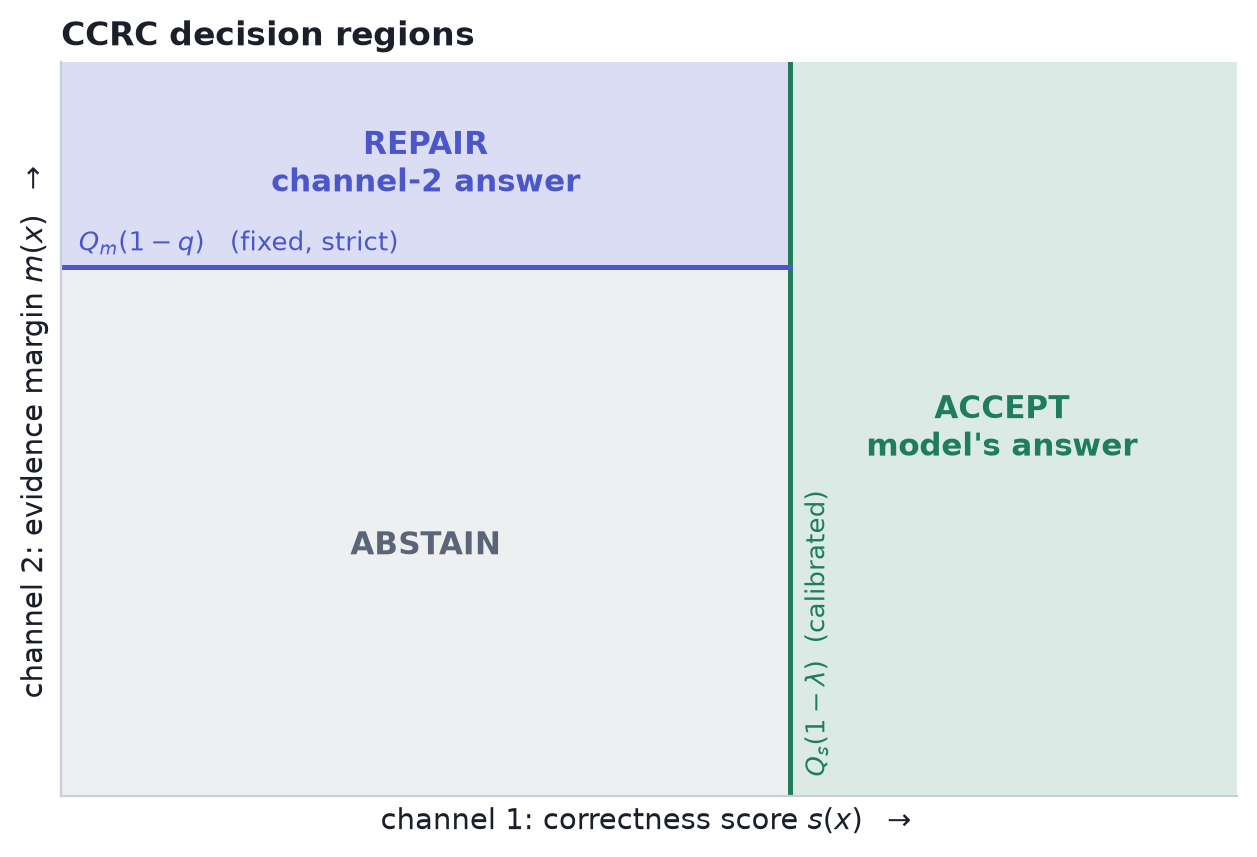
\includegraphics[width=0.55\textwidth]{fig_method.png}
\caption{The $(s,m)$ plane under policy \eqref{eq:policy}. The acceptance threshold moves along the
sequence; the repair gate is fixed, so the accepted region grows while the repair region shrinks.}
\label{fig:method}
\end{figure}

\subsection{How thresholds and gate are fixed}
\label{sec:fixing}

Both are values, and both are computed from the fit fold, which is disjoint from the calibration
fold and from the test fold.
\begin{itemize}
\item \emph{Score grid.} The channel-1 model is fitted on the fit fold. Its out-of-fold scores on
  that fold (image-grouped five-fold cross-fitting inside the fit fold) define the grid
  $t_j=Q_{1-\lambda_j}$ of their empirical distribution, with $\lambda_1<\dots<\lambda_{40}=1$
  equally spaced. Using out-of-fold scores keeps the quantile-to-value map faithful to
  out-of-sample behaviour; an in-sample fit is mildly overconfident on its own data.
\item \emph{Start.} The first hypothesis is where $c\,k_{\mathrm{start}}(e_0)$ items are expected
  to be emitted, $\lambda_1=\min\{0.9,\max\{0.05,\,c\,k_{\mathrm{start}}(e_0)/n_{\mathrm{cal}}\}\}$,
  with $k_{\mathrm{start}}(e_0)=\min\{k:U(e_0,k;\delta)\le\alpha\}$ the smallest emitted count at
  which $e_0$ observed errors still certify the target (Lemma~\ref{lem:kstart}). The default is
  $e_0=1$, $c=1.5$: start where one error can be tolerated, with half as much again as headroom for
  fold-to-fold variation in $K$. The start is computed from $\alpha$, $\delta$ and $n_{\mathrm{cal}}$
  alone, before any label is read; \S\ref{sec:start} ablates it.
\item \emph{Repair gate.} $g=Q_{1-q}(m)$ over grounded fit-fold items. Three ways of fixing
  $q$ keep the guarantee: (a) \emph{external}: $q$ is chosen once on a different benchmark by
  running the same procedure there and keeping the candidate (filtering, or $q\in\{0.05,0.10,0.25,0.50\}$)
  that certifies the most coverage; (b) \emph{fit-fold}: the same choice is made inside each split on the fit
  fold alone; (c) \emph{union}: three gates $\{0.05,0.10,0.25\}$ are each certified at $\delta/3$ and
  the certified policy with the largest calibration coverage is emitted.
\end{itemize}

\subsection{Validity}
\label{sec:validity}

\begin{theorem}[CCRC validity]
\label{thm:validity}
Under Assumptions~\ref{ass:iid} and~\ref{ass:family}, let $\hat\jmath$ be the last index passed by the
fixed-sequence test that proceeds through $j=1,2,\dots$ while $U(V_j,K_j;\delta)\le\alpha$ on the
calibration sample and stops at the first failure ($\hat\jmath=0$ if the first test fails, in which
case nothing is emitted). Then
\[
\Pr\bigl[\Risk(\pi_{\hat\jmath})\le\alpha\bigr]\ \ge\ 1-\delta,
\]
where the probability is over the calibration sample, conditional on the fit data.
\end{theorem}

\begin{proof}
Condition on the fit data, so the policies are fixed. For policy $j$ let $K_j=\sum_i\emit_j(X_i)$ and
$V_j=\sum_iW_j(Z_i)$, and consider $H_j:\Risk(\pi_j)>\alpha$. Emission is a function of $X$ alone.
By Assumption~\ref{ass:iid} the units are independent, so conditional on the set of emitted units
(equivalently, on the emission pattern), the emitted units are i.i.d.\ draws from $P(\cdot\mid\emit_j=1)$
and each has error indicator $W_j\sim\mathrm{Bernoulli}(\Risk(\pi_j))$, independently across units.
Hence $V_j\mid\{K_j=k\}\sim\mathrm{Bin}(k,\Risk(\pi_j))$, and by construction of the
Clopper--Pearson bound, $\Pr[U(V_j,K_j;\delta)\le\alpha\mid K_j=k]\le\delta$ whenever
$\Risk(\pi_j)>\alpha$ and $k\ge1$; for $k=0$ the bound is $1>\alpha$. So $\phi_j=\ind{U\le\alpha}$ is a
level-$\delta$ test of $H_j$.

Let $j_0=\min\{j:H_j\text{ is true}\}$, if it exists. The sequence reaches an index $\ge j_0$ only if $H_{j_0}$
is rejected, an event of probability at most $\delta$. On the complement, $\hat\jmath<j_0$, so every
index the procedure can return has $\Risk(\pi_{\hat\jmath})\le\alpha$. If no $H_j$ is true the claim is
trivial, and $\hat\jmath=0$ emits nothing and has risk $0$ by convention.
\end{proof}

The proof uses neither monotonicity of the risk along the sequence nor nesting of the emitted sets;
nesting is what makes ``the last index that passed'' a coverage-maximising return. It also does not
use whether $W_j$ refers to the model's answer or to channel 2's, which is why Proposition~\ref{prop:floor}
does not bind: its premise restricts the action space, and the certificate never refers to it.

\begin{corollary}[Gate fixed on other data, or chosen on the fit fold]
\label{cor:gate}
If $g$ is a constant, is computed from external data independent of the calibration sample, or is
computed from the fit data (including by a selection rule applied to the fit data alone), the policy
family satisfies Assumption~\ref{ass:family} and Theorem~\ref{thm:validity} holds at the full level
$\delta$.
\end{corollary}

\begin{corollary}[Union over a pre-specified set of gates]
\label{cor:union}
Let $\mathcal Q$ be a finite set of gate values fixed in advance. Run the fixed-sequence test for each at
level $\delta/|\mathcal Q|$ and emit any certified policy, chosen by any rule that may use the calibration
sample. Then the emitted policy has risk at most $\alpha$ with probability at least $1-\delta$.
\end{corollary}
\begin{proof}
By Theorem~\ref{thm:validity} each family fails with probability at most $\delta/|\mathcal Q|$; on the
complement of the union of these events every certified policy is compliant.
\end{proof}

A gate chosen by looking at the calibration or test outcomes of the benchmark under evaluation is not
covered by either corollary. Section~\ref{sec:main} reports the continuity gate $q=0.10$, which was selected in exploratory runs on these benchmarks, as an
\emph{uncertified} reference arm.

\begin{lemma}[Minimal certifiable emitted set]
\label{lem:kstart}
$U(0,k;\delta)=1-\delta^{1/k}$, so $e_0=0$ errors certify $\alpha$ iff
$k\ge k_{\mathrm{start}}(0)=\lceil\ln\delta/\ln(1-\alpha)\rceil$, which is $22$ at $\alpha=\delta=0.10$.
For $e_0\ge1$, $k_{\mathrm{start}}(e_0)$ is the smallest $k$ with $\Pr[\mathrm{Bin}(k,\alpha)\le e_0]\le\delta$;
at $\alpha=\delta=0.10$ it is $38,52,65$ for $e_0=1,2,3$, and at $\delta/3$ it is $33,51,66,81$ for $e_0=0,\dots,3$.
\end{lemma}
\begin{proof}
$\Pr[\mathrm{Bin}(k,p)\le e_0]$ is decreasing in $p$ and equals $\delta$ at $p=U(e_0,k;\delta)$, so
$U(e_0,k;\delta)\le\alpha$ iff $\Pr[\mathrm{Bin}(k,\alpha)\le e_0]\le\delta$. For $e_0=0$ this is
$(1-\alpha)^k\le\delta$.
\end{proof}

Starting the sequence at $e_0=0$ makes the first test fail if a single error falls in the first
emitted set, and because the sequence stops at the first failure, that is an abort. An analytic start
at $e_0\ge1$ removes this sensitivity to one error but places the first hypothesis at a more
permissive threshold, which a weak score may fail for a different reason. Neither is better in
general, which is why \S\ref{sec:start} reports the whole range.

\subsection{Clustered units}
\label{sec:clusters}

When an image carries several questions, the item is not an i.i.d.\ unit; the image is. Two exact
options exist. If calibration uses one item drawn uniformly at random from each of $n$ i.i.d.\ images,
the units are i.i.d.\ and Theorem~\ref{thm:validity} applies to the risk under that sampling
scheme, which equals the item-level risk when images have equal numbers of items. If calibration uses all
items, positive within-image correlation of errors makes $V_j\mid K_j$ over-dispersed relative to the
binomial and the bound is anti-conservative by an amount that grows with the intra-image
correlation; \S\ref{sec:validity-audit} measures this in a known-population simulation and
\S\ref{sec:protocol} measures the correlation in the data we use.

\subsection{The rank-indexed variant}
\label{sec:rank}

An implementer who has no pre-specified grid takes thresholds as quantiles of the calibration
sample itself, $t_j=Q_{1-\lambda_j}(s_{\mathrm{cal}})$, and a repair gate $g=Q_{1-q}(m_{\mathrm{cal}})$. Selecting the top
$\lceil\lambda n\rceil$ items by score makes $K$ deterministic and makes the emitted set a function of all calibration
features jointly; then $V$ is Poisson-binomial rather than binomial and the argument above does not apply.
We treat this variant as the conventional baseline and quantify its behaviour in
\S\ref{sec:ladder} and \S\ref{sec:validity-audit}, without claiming a theorem for it.

\begin{algorithm}[t]
\caption{CCRC. Folds $\mathcal D_{\mathrm{fit}},\mathcal D_{\mathrm{cal}}$ are disjoint and unions of images; $\alpha,\delta,e_0,c$ are fixed in advance.}
\label{alg:ccrc}
\begin{algorithmic}[1]
\State fit $s$ on $\mathcal D_{\mathrm{fit}}$; compute out-of-fold scores $\tilde s$ on $\mathcal D_{\mathrm{fit}}$
\State choose gate fraction $q$ (external, fit-fold, or union); $g\gets Q_{1-q}\{m_i:i\in\mathcal D_{\mathrm{fit}}\}$
\State $\lambda_1\gets\min\{0.9,\max\{0.05,\,c\,k_{\mathrm{start}}(e_0)/|\mathcal D_{\mathrm{cal}}|\}\}$; $t_j\gets Q_{1-\lambda_j}(\tilde s)$, $j=1..M$
\State $\hat\jmath\gets0$
\For{$j=1$ \textbf{to} $M$}
  \State $A\gets\{i\in\mathcal D_{\mathrm{cal}}:s_i\ge t_j\}$, $R\gets\{i\notin A:m_i\ge g\}$; $K\gets|A|+|R|$
  \State $V\gets\sum_{A}(1-Y_i)+\sum_{R}(1-Y^{(2)}_i)$
  \If{$K>0$ \textbf{and} $U(V,K;\delta)\le\alpha$} $\hat\jmath\gets j$ \Else\ \textbf{break} \EndIf
\EndFor
\State \textbf{deploy:} if $\hat\jmath=0$ abstain everywhere; else accept if $s(x)\ge t_{\hat\jmath}$, repair if $m(x)\ge g$, abstain otherwise
\end{algorithmic}
\end{algorithm}

\section{Experimental protocol}
\label{sec:protocol}

\paragraph{Models, benchmarks and signals.}
Backbones are LLaVA-1.5-7B \citep{llava} in 4-bit, Qwen2-VL-2B-Instruct \citep{qwenvl}, and LLaVA decoded with
visual contrastive decoding \citep{vcd}. Channel 2 is OWLv2-base \citep{owlv2} with $\theta=0.15$. Benchmarks are
the POPE adversarial split \citep{pope} and the AMBER discriminative benchmark \citep{amber}; MME, GQA and
HallusionBench appear only where the detector does not apply (\S\ref{sec:noevidence}). Per-item signals were
extracted once and are released, so every analysis below runs on a CPU. The extended POPE and AMBER cells (items $1500$--$2999$ of the
POPE adversarial split and items $500$--$2999$ of the shuffled AMBER list) were extracted with the same prompts and detector query as the
earlier cells; in the AMBER extension, photographs larger than $2000$ pixels on the long side were shrunk before detection because the
detector's preprocessing of the largest ones ($54$ megapixels) exhausted host memory.

\paragraph{Cohorts and the unit of splitting.}
The extraction streamed the first $N$ rows of each public benchmark. We recovered the image identifier of every
item from the benchmark metadata and verified the reconstruction against the cached gold labels, object phrases
and categories (all agree). Table~\ref{tab:cohort} reports what enters each cell. The POPE items are
six questions per image (three present, three absent objects), so there are $75$, $100$, $250$ and $500$ distinct
images in the four POPE cell sizes; the smaller POPE cells are subsets of the largest one's images, and POPE-3000 is the whole
adversarial split. AMBER contributes $3.1$ items per image over $957$ images. Folds are unions of whole images, drawn at
random with a third of the images per fold. The intra-image correlation of the model's errors is slightly \emph{negative}
($-0.01$ to $-0.09$): in POPE the balanced yes/no design makes an error on one question of an image mildly predictive of a
correct answer on another.

\begin{table}[t]
\centering
\caption{Cohort flow. ``Detector value'' is the number of items for which the detector returned a score; the
remaining items stay in every analysis, keep the channel-1 decision, and cannot be repaired. In POPE the
exclusions are object phrases the extraction script failed to parse (POPE contains the typo ``imange''); in AMBER
they are the attribute and relation queries, which name no object. ICC is the intra-image correlation of the
model's errors.}
\label{tab:cohort}
\small
\resizebox{\textwidth}{!}{\begin{tabular}{lrrrrrlcc}
\toprule
Setting & items & images & items/img & ICC & detector value & excluded from the grounded cohort & images/fold & $\mu$ (\%)\\
\midrule
POPE-1500, LLaVA & 1500 & 250 & 6.0 & $-$0.04 & 1500 & 0 unparsed object phrases & 83/83/84 & 18.1\\
POPE-adv, LLaVA & 450 & 75 & 6.0 & $-$0.05 & 444 & 6 unparsed object phrases & 25/25/25 & 17.3\\
POPE-adv, Qwen2-VL & 600 & 100 & 6.0 & $-$0.04 & 591 & 9 unparsed object phrases & 33/33/34 & 12.7\\
POPE-adv, LLaVA+VCD & 600 & 100 & 6.0 & $-$0.04 & 591 & 9 unparsed object phrases & 33/33/34 & 19.7\\
AMBER(d), LLaVA & 500 & 392 & 1.3 & $-$0.09 & 228 & 272 attribute/relation queries & 130/130/132 & 21.4\\
\bottomrule
\end{tabular}
}
\end{table}

\paragraph{Primary analysis and missing evidence.}
The primary cohort contains all items. Items with no detector value receive zeroed grounding features and a
missing-evidence flag in the score, and a margin $m=-1$ so they are never repaired. A secondary analysis restricted to
items with a detector value appears in Appendix~\ref{app:grounded}. Excluding the items would analyse the
detector's coverage; a deployed system must decide what to do with a question the detector cannot parse.

\paragraph{Procedure.}
Each split draws three image-disjoint folds (fit, calibration, test); the score is a logistic regression with five
features (the VLM's probability, its confidence margin, the detector score, the detector score signed by the VLM's
answer, and the missing flag); thresholds and gate are fixed from the fit fold as in \S\ref{sec:fixing}; the
fixed-sequence test uses Clopper--Pearson bounds at $\delta=0.10$; and the deployed policy is evaluated on the test fold.
We use $400$ paired splits per cell, so every arm in a comparison sees identical folds.

\paragraph{Uncertainty.}
Repeated random splits of one benchmark measure how sensitive the procedure is to the split. They do not
measure how the result would change on a fresh benchmark: the interval over splits shrinks like $1/\sqrt{\text{splits}}$ while
uncertainty about the dataset does not shrink at all. We therefore report gains as the mean over the $400$ splits
with a $95\%$ percentile interval from an \emph{outer image-level bootstrap}: $300$ bootstrap datasets
are drawn by resampling images with replacement, the full protocol is run on each with $20$ splits, and the
interval is taken over bootstrap datasets. A duplicated image keeps its identifier and is always placed in one fold. Because a
bootstrap dataset contains only about $63\%$ distinct images, the interval is somewhat wider than the one a
fresh sample of the same size would give. We do not report $p$-values over splits.

\paragraph{Validity audits.}
Realised test-fold risk carries binomial noise and cannot audit a population guarantee: a policy whose true risk is
$0.08$ exceeds $0.10$ on a $150$-item test fold with substantial probability. We report two statistics per
cell. \emph{exc} is the fraction of non-aborted splits whose test-fold risk exceeds $\alpha$; under validity it
is bounded by $\delta$ plus finite-fold noise. \emph{cv} is the fraction of splits for which the one-sided
$90\%$ Clopper--Pearson \emph{lower} bound on the test-fold risk exceeds $\alpha$ (a confident violation); if the
population risk is at most $\alpha$ it is at most $0.1$ per split by the same argument as the theorem. Test folds
are used for nothing else: no score, threshold, gate or start is selected on them. An exact audit requires a known
population, which the simulation in \S\ref{sec:validity-audit} provides.

\section{Results}
\label{sec:results}

\subsection{Certified coverage}
\label{sec:main}

Table~\ref{tab:main} compares CCRC with filtering on identical folds at $\alpha\in\{0.10,0.15\}$,
$\delta=0.10$, all items, and Figure~\ref{fig:forest} plots the gains with their bootstrap intervals. Three
certified gate variants appear. In the \emph{external} variant the gate fraction $q$ is a constant chosen once on a
different benchmark (AMBER for the POPE cells, POPE-3000 for AMBER), by running the same protocol there on random
subsamples whose calibration fold has the \emph{target's} size and keeping the candidate (filtering, or
$q\in\{0.05,0.10,0.25,0.50\}$) with the highest mean certified coverage. The choice is $q=0.05$ for
the small cells at $\alpha=0.10$, the small LLaVA cell at $0.15$ and POPE-1500 at $0.10$ ($q=0.05$ in five of the twelve combinations) and $q=0.5$ in the other seven. In the \emph{fit-fold}
variant $q$ is chosen inside each split on the fit fold, with filtering as one candidate. A third variant
(\emph{external, full-size}) treats the whole development benchmark as a single calibration sample; it is
reported in the last column of Table~\ref{tab:main} because it shows what picking the gate at the wrong
sample size costs. The size-matched variant was defined after we saw that the full-size variant loses on the small cells, so
the comparison between them is exploratory and the size-matched rule should be read as a recommendation.

\begin{table}[t]
\centering
\caption{Certified coverage (\%), with the abort rate (\%) in parentheses, $\delta=0.10$, $400$ paired
splits, all-item cohort. Gain is the mean paired difference over splits against filtering; the interval is the
$95\%$ percentile interval from the outer image-level bootstrap (\S\ref{sec:protocol}), and
$P(\text{gain}>0)$ is the fraction of bootstrap datasets with a positive gain. The last column is the gain with the
gate chosen on the development benchmark at its full size.}
\label{tab:main}
\scriptsize
\resizebox{\textwidth}{!}{\begin{tabular}{lcccccccc}
\toprule
 & & Filter & \multicolumn{3}{c}{CCRC, external gate} & & \multicolumn{2}{c}{CCRC, fit-fold gate}\\
\cmidrule(lr){4-6}\cmidrule(lr){8-9}
Setting & $\alpha$ & cov.\ (abort) & cov.\ (abort) & gain [95\% CI] & $P(\text{gain}>0)$ & & cov.\ (abort) & gain [95\% CI]\\
\midrule
POPE-1500, LLaVA & 0.10 & 68.2 (0) & 77.6 (0) & +9.4 [$-$4.9, +20.7] & 0.90 & 77.0 (1) & +8.8 [$-$8.0, +18.8]\\
 & 0.15 & 85.5 (0) & 92.8 (0) & +7.3 [+4.2, +11.0] & 1.00 & 92.6 (0) & +7.1 [+3.6, +10.7]\\
\addlinespace
POPE-3000, LLaVA & 0.10 & 76.6 (0) & 83.2 (0) & +6.6 [$-$1.0, +10.7] & 0.97 & 82.8 (0) & +6.3 [$-$2.3, +9.8]\\
 & 0.15 & 90.8 (0) & 95.8 (0) & +5.1 [+2.9, +7.1] & 1.00 & 95.8 (0) & +5.0 [+2.7, +7.0]\\
\addlinespace
POPE-adv, LLaVA & 0.10 & 44.5 (25) & 37.3 (48) & $-$7.2 [$-$24.4, +18.4] & 0.50 & 41.4 (34) & $-$3.1 [$-$13.8, +9.3]\\
 & 0.15 & 72.5 (2) & 82.6 (2) & +10.1 [$-$3.5, +34.8] & 0.94 & 82.0 (2) & +9.4 [$-$3.3, +28.8]\\
\addlinespace
POPE-adv, Qwen2-VL & 0.10 & 76.9 (1) & 69.1 (14) & $-$7.7 [$-$33.7, +15.4] & 0.37 & 71.2 (10) & $-$5.7 [$-$25.1, +10.5]\\
 & 0.15 & 94.6 (0) & 95.7 (0) & +1.1 [$-$9.8, +13.2] & 0.78 & 95.0 (0) & +0.4 [$-$7.5, +8.9]\\
\addlinespace
POPE-adv, LLaVA+VCD & 0.10 & 45.8 (14) & 33.5 (46) & $-$12.3 [$-$26.5, +12.5] & 0.23 & 39.6 (30) & $-$6.2 [$-$13.4, +8.9]\\
 & 0.15 & 74.4 (0) & 76.8 (0) & +2.4 [$-$12.7, +22.2] & 0.82 & 76.1 (0) & +1.7 [$-$10.3, +17.6]\\
\addlinespace
AMBER(d), LLaVA & 0.10 & 64.4 (0) & 67.5 (0) & +3.1 [$-$14.5, +4.9] & 0.60 & 66.8 (1) & +2.4 [$-$12.5, +4.4]\\
 & 0.15 & 75.7 (0) & 79.6 (0) & +3.9 [+2.6, +8.3] & 1.00 & 79.5 (0) & +3.8 [$-$0.4, +8.1]\\
\bottomrule
\end{tabular}
}
\end{table}

\begin{figure}[t]
\centering
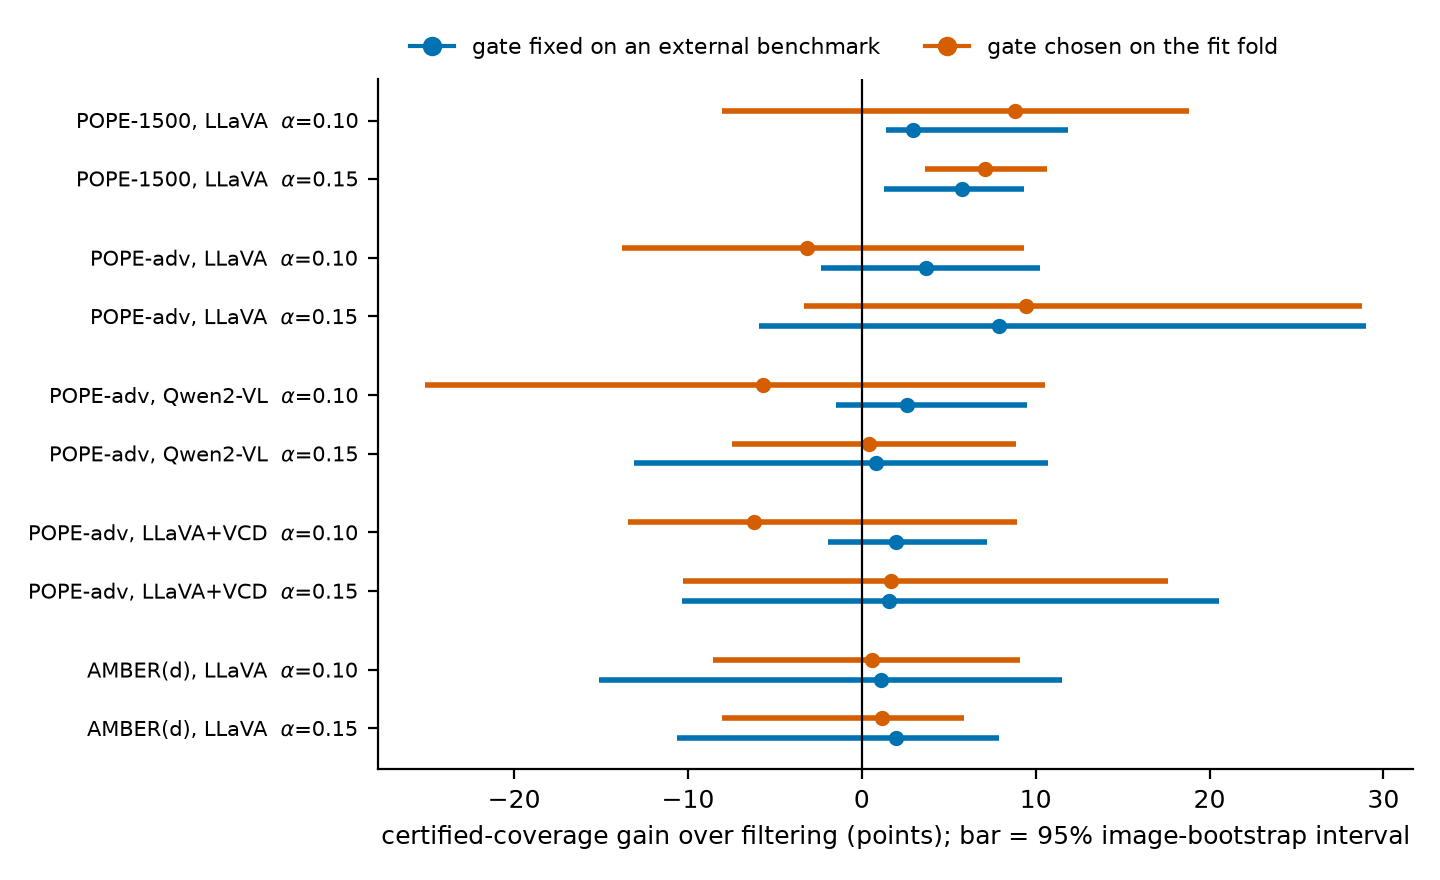
\includegraphics[width=0.9\textwidth]{fig_forest.png}
\caption{Gain in certified coverage over filtering. Points are means over $400$ splits of the original
benchmark; bars are $95\%$ image-bootstrap intervals.}
\label{fig:forest}
\end{figure}

With the size-matched external gate the gain is positive in all twelve (cell, $\alpha$) combinations, from $+0.8$ to
$+7.3$ points, and the share of bootstrap datasets with a positive gain is $0.60$--$1.00$. The $95\%$
interval excludes zero in seven of the twelve: POPE-1500 and POPE-3000 at $\alpha=0.15$, POPE-1500 at $0.10$, AMBER at $0.15$, and
three of the small cells, where the gain is $+1.2$ to $+1.8$ points with intervals whose lower end is within $0.15$ points of zero. The larger
gains occur where the calibration folds are large and the gate is $q=0.5$: $+6.6$ and $+5.1$ points on
POPE-3000 (folds of about $1000$ items, $166$ images), $+7.3$ on POPE-1500 at $\alpha=0.15$ and $+3.9$ on AMBER
at $\alpha=0.15$. On the small cells the selected gate is $q=0.05$, which repairs $0.2$--$0.7\%$ of test items and
gains about one point; the per-split standard deviations of the gain are $1.3$--$11$ points.

The fit-fold gate is more flexible and more variable: $+8.8$ and $+7.1$ points on POPE-1500 and $+6.3$, $+5.0$ on POPE-3000,
but between $-6.2$ and $+9.4$ on the small cells, negative in all three at $\alpha=0.10$, because a gate chosen
on a fit fold of $150$ items is itself noisy and a wrong choice costs more than the right one returns. The union over
three gates avoids selection noise and pays $\delta/3$ per gate: it gains $+2.0$ to $+4.4$ points on the
cells with $500$ or more calibration items and loses up to $16.5$ points on those with $150$--$200$
(Appendix~\ref{app:audit}). The full-size external gate ($q=0.5$ for every POPE cell) loses $7.2$, $7.7$ and
$12.3$ points on the three small cells at $\alpha=0.10$ and $5.5$ on AMBER at $0.10$, and gains up to $+10.1$ elsewhere. The continuity gate $q=0.10$,
selected in exploratory runs on these benchmarks, gains $0.0$ to $+3.9$ points; we report it as an uncertified reference arm
and do not use it for any claim, since a gate chosen with knowledge of the benchmarks is what
Theorem~\ref{thm:validity} does not cover.

\begin{figure}[t]
\centering
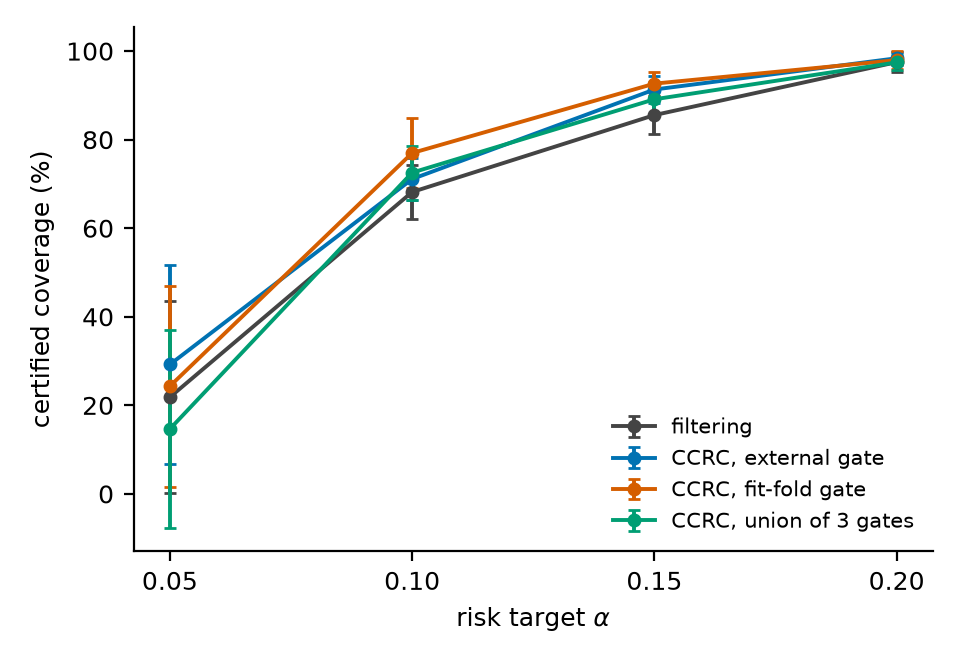
\includegraphics[width=0.55\textwidth]{fig_alpha.png}
\caption{Certified coverage against the risk target on POPE-3000. Bars are one standard deviation over
splits.}
\label{fig:alpha}
\end{figure}

Coverage rises with $\alpha$ for every arm (Figure~\ref{fig:alpha}), and the gap between CCRC and filtering is
largest at moderate targets. The audit columns of Appendix Table~\ref{tab:audit} are discussed in
\S\ref{sec:validity-audit}.

\subsection{What each protocol change does}
\label{sec:ladder}

Table~\ref{tab:ladder} introduces the changes one at a time, from a conventional implementation (item-level folds,
thresholds and gate as quantiles of the calibration fold, a start at $k_{\mathrm{start}}(0)$ and a fixed $q=0.10$) to the
protocol of this paper; the $\alpha=0.15$ version is in Appendix~\ref{app:ladder}.

\begin{table}[t]
\centering
\caption{Filtering / CCRC certified coverage (\%) at $\alpha=0.10$ as the protocol changes. Rungs L0--L3 use the
fixed gate $q=0.10$, rung L4 chooses the gate on the fit fold, and rung L5 keeps items with no detector
value. L0--L4 use the grounded cohort of each cell; L5 uses all items, so
its absolute level for AMBER is lower: the attribute and relation queries are harder and cannot be repaired.}
\label{tab:ladder}
\small
\resizebox{\textwidth}{!}{\begin{tabular}{lccccc}
\toprule
 & POPE-1500,\ LLaVA & POPE-adv,\ LLaVA & POPE-adv,\ Qwen2-VL & POPE-adv,\ LLaVA+VCD & AMBER(d),\ LLaVA\\
\midrule
conventional protocol (item folds, calibration quantiles, $e_0{=}0$, fixed $q{=}0.10$) & 68.6/71.8 & 44.0/47.1 & 77.9/79.7 & 48.8/51.0 & 91.8/81.6\\
+ image-grouped folds & 68.2/71.3 & 43.1/48.3 & 77.6/79.5 & 47.9/50.8 & 92.0/81.9\\
+ fixed value grid and gate (fit fold) & 67.5/70.9 & 35.0/42.3 & 75.5/77.7 & 39.9/45.3 & 90.9/85.1\\
+ analytic start $e_0{=}1$ & 68.2/71.1 & 43.6/47.4 & 75.6/78.0 & 45.5/47.6 & 90.2/90.0\\
+ gate chosen on the fit fold & 68.2/77.0 & 43.6/39.4 & 75.6/68.3 & 45.5/39.7 & 90.2/89.8\\
+ all-item cohort & 68.2/77.0 & 44.5/41.4 & 76.9/71.2 & 45.8/39.6 & 55.2/55.8\\
\bottomrule
\end{tabular}
}
\end{table}

Image-grouped folds change coverage by at most $1.2$ points on the POPE cells and lower the test-fold exceedance on the five
POPE cells from $0.14, 0.10, 0.11, 0.16, 0.12$ to $0.10, 0.08, 0.09, 0.09, 0.12$. Replacing calibration quantiles by fit-fold
values costs coverage when the fixed sequence starts at $e_0=0$: the first hypothesis lands at a threshold where a single error
aborts the test, and the abort rate of filtering on POPE-adv LLaVA rises from $18\%$ to $34\%$; the analytic start at $e_0=1$
recovers most of it. The gain of repair over filtering on the large POPE cells is stable under L0--L3 ($+2.9$ to $+3.5$ points
on POPE-1500, $+2.0$ on POPE-3000). The largest effect of the protocol is on AMBER, where the conventional protocol makes CCRC
abort on $72\%$ of splits (coverage $26.2\%$ against $91.0\%$ for filtering); image-grouped folds, value-indexed thresholds and
the analytic start remove it in turn ($34.7\%$, $78.3\%$, $90.1\%$), and the fit-fold gate gives $93.3\%$ against $90.9\%$. The loss
that a conventional protocol attributes to repair on AMBER is therefore a property of the start of the fixed sequence.

\subsection{What a repair is}
\label{sec:accounting}

A natural question for any correction method is how often it changes the model's answer, and whether
the changes are right. Table~\ref{tab:acct} separates the repaired items (those emitted through channel 2) into
those where channel 2's answer differs from the model's and those where the two agree, and counts wrong-to-right and
right-to-wrong changes.

\begin{table}[t]
\centering
\caption{Accounting of repaired items, external-gate variant, all items, pooled over test folds of $400$ splits.
``Repaired'' and ``answer changed'' are percentages of test items; the next five columns are percentages of repaired
items. ``FP corrected'' is the number of the model's false-positive errors (it said yes, gold is no) whose emitted answer was
corrected, over the number of such errors; ``FN corrected'' is the share of the model's false-negative errors corrected.}
\label{tab:acct}
\small
\resizebox{\textwidth}{!}{\begin{tabular}{lccccccccccc}
\toprule
 & & & \multicolumn{2}{c}{\% of test items} & \multicolumn{5}{c}{\% of repaired items} & & \\
\cmidrule(lr){4-5}\cmidrule(lr){6-10}
Setting & $\alpha$ & $q$ & repaired & answer changed & changed & wrong$\to$right & right$\to$wrong & agree, right & agree, wrong & FP corrected & FN corrected (\%)\\
\midrule
POPE-1500, LLaVA & 0.10 & 0.5 & 11.97 & 6.02 & 50 & 43 & 7.8 & 46 & 4.1 & 840/11420 & 37.6\\
 & 0.15 & 0.5 & 6.42 & 4.21 & 65 & 57 & 8.2 & 32 & 2.5 & 579/11482 & 27.4\\
\addlinespace
POPE-3000, LLaVA & 0.10 & 0.5 & 10.08 & 5.72 & 57 & 46 & 11.0 & 40 & 3.0 & 1024/20516 & 36.3\\
 & 0.15 & 0.5 & 4.58 & 2.92 & 64 & 56 & 7.8 & 34 & 2.3 & 641/20516 & 20.1\\
\addlinespace
POPE-adv, LLaVA & 0.10 & 0.5 & 13.05 & 4.46 & 34 & 28 & 6.4 & 60 & 5.5 & 144/2086 & 29.3\\
 & 0.15 & 0.5 & 8.24 & 3.09 & 38 & 35 & 3.0 & 58 & 4.0 & 277/3826 & 21.8\\
\addlinespace
POPE-adv, Qwen2-VL & 0.10 & 0.5 & 8.93 & 2.50 & 28 & 19 & 8.5 & 65 & 7.4 & 0/2364 & 18.5\\
 & 0.15 & 0.5 & 1.43 & 0.47 & 33 & 26 & 7.1 & 53 & 13.6 & 0/2724 & 4.0\\
\addlinespace
POPE-adv, LLaVA+VCD & 0.10 & 0.5 & 13.43 & 3.53 & 26 & 19 & 7.5 & 65 & 9.1 & 466/5815 & 22.0\\
 & 0.15 & 0.5 & 6.96 & 2.80 & 40 & 30 & 10.3 & 52 & 7.8 & 864/10477 & 15.2\\
\addlinespace
AMBER(d), LLaVA & 0.10 & 0.5 & 4.37 & 2.38 & 54 & 51 & 3.6 & 35 & 10.5 & 1461/34791 & 12.5\\
 & 0.15 & 0.5 & 3.34 & 2.12 & 64 & 60 & 3.1 & 30 & 6.8 & 1467/34989 & 11.1\\
\bottomrule
\end{tabular}
}
\end{table}

The accounting depends strongly on the gate. With the small gate ($q=0.05$, selected on the cells with $150$--$200$ calibration items at
$\alpha=0.10$) the repaired mass is $0.2$--$0.9\%$ of test items and the answer is changed for $0.0$--$0.45\%$; on POPE-adv Qwen2-VL
the detector agrees with the model on all repaired items and no answer changes. With the large gate ($q=0.5$) the repaired mass
is $4.4\%$ (AMBER) to $10.1\%$ (POPE-3000) of test items at $\alpha=0.10$ and the answer changes for $2.4$--$5.7\%$. Among repaired items the
detector agrees with the model on $22$--$100\%$ at $\alpha=0.10$: those items are \emph{re-emitted with detector confirmation},
which is a different benefit from correction: an item the correctness score would have abstained on is emitted
because a distinct source confirms it. Where the answer is changed it is mostly right: $18{,}583$ wrong-to-right against
$4{,}486$ right-to-wrong changes on POPE-3000 ($81\%$) and $8{,}830$ against $634$ on AMBER ($93\%$), while with $q=0.05$ the
right-to-wrong count is zero in every cell. A larger gate corrects more and makes more mistakes, and the certificate prices the mixture.
False-positive errors are corrected only with the large gate: $1{,}024$ of $20{,}516$ ($5.0\%$) on POPE-3000 and $1{,}461$ of $34{,}791$ ($4.2\%$) on
AMBER, none with $q=0.05$; $0$ to $36.3\%$ of the model's false-negative errors are corrected, the highest share on POPE-3000.

Table~\ref{tab:sym} repeats the accounting for one-sided and polarity-symmetric gates, each gating a fixed
fraction $q=0.10$ of its own polarity's margins. The symmetric gate admits negative-polarity repairs, which are
highly precise, and these confirm the model's own ``no'' answers; they change an answer for $8$ false positives on AMBER and
none on the POPE cells. The reason is structural in this instantiation: the model's false positives are items where the detector
also fires, so the detector's strongly negative evidence occurs on items the model already got right.

\begin{table}[t]
\centering
\caption{Gate polarity at $\alpha=0.10$, $q=0.10$ per polarity. Gain over filtering in points, repaired items as a
percentage of test items, and the number of false-positive errors corrected (pooled over $400$ test folds).
Pooled margin is the gate used elsewhere in the paper.}
\label{tab:sym}
\small
\resizebox{\textwidth}{!}{\begin{tabular}{lcccccccccccc}
\toprule
 & \multicolumn{3}{c}{pooled margin (CCRC)} & \multicolumn{3}{c}{positive only} & \multicolumn{3}{c}{negative only} & \multicolumn{3}{c}{symmetric}\\
\cmidrule(lr){2-4}\cmidrule(lr){5-7}\cmidrule(lr){8-10}\cmidrule(lr){11-13}
Setting & gain & rep.\ \% & FP fixed & gain & rep.\ \% & FP fixed & gain & rep.\ \% & FP fixed & gain & rep.\ \% & FP fixed\\
\midrule
POPE-1500, LLaVA & +2.9 & 1.88 & 0 & +1.3 & 0.80 & 0 & +0.2 & 0.07 & 0 & +1.4 & 0.87 & 0\\
POPE-adv, LLaVA & +3.7 & 1.93 & 0 & +1.6 & 0.61 & 0 & +0.8 & 0.14 & 0 & +2.1 & 0.76 & 0\\
POPE-adv, Qwen2-VL & +2.6 & 0.90 & 0 & +1.0 & 0.40 & 0 & +2.5 & 0.20 & 0 & +3.2 & 0.59 & 0\\
POPE-adv, LLaVA+VCD & +2.0 & 0.68 & 0 & +0.8 & 0.19 & 0 & +0.9 & 0.21 & 0 & +1.5 & 0.40 & 0\\
AMBER(d), LLaVA & +2.5 & 2.84 & 0 & +1.1 & 0.61 & 0 & +0.1 & 0.03 & 0 & +1.1 & 0.64 & 0\\
\bottomrule
\end{tabular}
}
\end{table}

\paragraph{Where the gain comes from.}
Repaired items are themselves emitted, so whenever the certified threshold does not move the gain equals the repaired mass at filtering's own threshold; a dilution term appears when repairs lower the emitted risk and let the threshold open further. The threshold differs between the two arms on $3$--$34\%$ of splits and the dilution term is $0.06$ to $1.5$ points; the automatic term is the larger one in ten of the twelve combinations (Appendix Table~\ref{tab:dilution}).

\subsection{The start of the sequence}
\label{sec:start}

Table~\ref{tab:start} varies the number of errors the first hypothesis can tolerate, $e_0\in\{0,1,2,3\}$ (so
$k_{\mathrm{start}}=22,38,52,65$), and the placement multiplier $c\in\{1.0,1.5\}$, for filtering and CCRC with the
fit-fold gate. On the three cells with at least $250$ images (POPE-1500, POPE-3000, AMBER) the choice is nearly irrelevant for
CCRC ($76.5$--$77.5\%$, $82.8$--$82.9\%$ and $66.7$--$67.1\%$) and moves filtering by at most $2.6$ points. On the three cells with
calibration folds of $150$--$200$ items filtering ranges from $22\%$ to $45\%$ (POPE-adv LLaVA), $23\%$ to $46\%$ (VCD) and
$73\%$ to $79\%$ (Qwen2-VL), with abort rates up to $67\%$, and CCRC follows. Neither extreme is good: $e_0=0$ makes the first test fail on
a single error; large $e_0$ together with $c=1.5$ places the first hypothesis at a permissive threshold at which the score does not
separate. We use $e_0=1$, $c=1.5$ throughout, fixed before the final runs and following the analytic argument of Lemma~\ref{lem:kstart};
the table shows it lies in a reasonable region and it was not selected on test outcomes. The practical consequence is that conclusions drawn on
calibration folds of $150$--$200$ items depend on the start of the sequence more than on the repair.

A search that spends part of $\delta$ on several starts, instead of committing to one, is also valid (Corollary~\ref{cor:union}). We tested the union over $e_0\in\{0,1,2\}$, each at $\delta/3$, choosing the certified policy with the largest calibration coverage (Appendix Table~\ref{tab:multistart}). It is below the single analytic start $e_0=1$ in all twelve combinations, by $0.7$ to $13$ points ($1$--$4$ points on the cells with $500$ or more calibration items, up to $13$ on the small ones), because the $\delta/3$ penalty exceeds what the extra starts recover.

\begin{table}[t]
\centering
\caption{Certified coverage (\%) and abort rate (\%) at $\alpha=0.10$ as the start of the fixed sequence varies,
filtering and CCRC with the fit-fold gate (Appendix~\ref{app:ladder} for $\alpha=0.05$ and $0.15$).}
\label{tab:start}
\scriptsize
\resizebox{\textwidth}{!}{\begin{tabular}{cccrrrrrrrrrr}
\toprule
 & & & \multicolumn{2}{c}{POPE-1500,~LLaVA} & \multicolumn{2}{c}{POPE-adv,~LLaVA} & \multicolumn{2}{c}{POPE-adv,~Qwen2-VL} & \multicolumn{2}{c}{POPE-adv,~LLaVA+VCD} & \multicolumn{2}{c}{AMBER(d),~LLaVA}\\
\cmidrule(lr){4-5}\cmidrule(lr){6-7}\cmidrule(lr){8-9}\cmidrule(lr){10-11}\cmidrule(lr){12-13}
$c$ & $e_0$ & $k_{\mathrm{start}}$ & filter & CCRC & filter & CCRC & filter & CCRC & filter & CCRC & filter & CCRC\\
\midrule
1.0 & 0 & 22 & 65.8 (4) & 76.5 (1) & 22.2 (54) & 33.8 (45) & 72.6 (5) & 64.6 (19) & 22.9 (50) & 29.9 (44) & 55.8 (0) & 47.5 (20)\\
1.0 & 1 & 38 & 68.3 (0) & 76.6 (1) & 41.2 (24) & 40.7 (32) & 76.5 (0) & 68.2 (13) & 42.8 (17) & 39.1 (30) & 55.8 (0) & 51.7 (12)\\
1.0 & 2 & 52 & 68.4 (0) & 76.9 (1) & 44.4 (24) & 41.8 (33) & 76.8 (0) & 71.5 (10) & 45.2 (15) & 39.0 (30) & 55.0 (2) & 54.3 (8)\\
1.0 & 3 & 65 & 68.2 (0) & 77.2 (0) & 44.0 (28) & 39.3 (40) & 76.0 (3) & 69.5 (13) & 45.3 (16) & 39.5 (31) & 54.3 (6) & 54.9 (10)\\
\addlinespace
1.5 & 0 & 22 & 67.5 (0) & 76.8 (1) & 36.9 (30) & 38.4 (36) & 76.5 (0) & 68.6 (14) & 39.5 (22) & 37.9 (32) & 55.7 (0) & 49.7 (15)\\
1.5 & 1 & 38 & 68.2 (0) & 77.0 (1) & 44.5 (25) & 41.4 (34) & 76.9 (1) & 71.2 (10) & 45.8 (14) & 39.6 (30) & 55.2 (3) & 55.8 (6)\\
1.5 & 2 & 52 & 68.4 (0) & 77.1 (1) & 38.5 (39) & 36.2 (45) & 77.1 (4) & 70.0 (14) & 43.8 (20) & 37.6 (35) & 52.6 (11) & 53.0 (14)\\
1.5 & 3 & 65 & 68.3 (0) & 77.5 (0) & 22.4 (67) & 22.2 (68) & 78.6 (2) & 73.7 (10) & 33.0 (45) & 29.4 (52) & 29.6 (54) & 30.8 (52)\\
\bottomrule
\end{tabular}
}
\end{table}

\subsection{Where the coverage comes from}
\label{sec:score}

\paragraph{The score.}
Table~\ref{tab:scores} compares scores under the same protocol, filtering only. The scorer of ConfLVLM \citep{conflvlm},
image--text similarity, certifies $0.5\%$ here at $\alpha=0.10$;
VLM confidence alone certifies $41.0\%$; a learned combination of the VLM's own signals $58.8\%$; adding
standardised image--text similarity does not help ($56.8\%$); adding detection grounding gives $68.2\%$ and the
lowest area under the risk--coverage curve ($0.0562$ against $0.0678$). Against the similarity scorer, CCRC with the external gate ($69.6\%$) gains $69.1$ points, of which $67.7$ come from the score and $1.4$ from certified
repair; with the fit-fold gate ($77.0\%$) the repair share is $8.8$ points. The correctness score is the dominant lever.

\begin{table}[t]
\centering
\caption{POPE-1500, filtering only: certified coverage (\%) with abort rate in parentheses, and area under the
risk--coverage curve at $\alpha=0.10$ (lower is better).}
\label{tab:scores}
\small
\begin{tabular}{lcccc}
\toprule
Score & $\alpha{=}0.05$ & $\alpha{=}0.10$ & $\alpha{=}0.15$ & AURC\\
\midrule
image--text similarity only (ConfLVLM scorer) & 0.0 (100) & 0.5 (94) & 3.4 (72) & 0.1621\\
VLM confidence only & 2.4 (93) & 41.0 (18) & 75.1 (5) & 0.0768\\
learned, VLM signals & 10.6 (61) & 58.8 (1) & 80.7 (0) & 0.0678\\
+ image--text similarity & 9.0 (67) & 56.8 (2) & 80.5 (0) & 0.0691\\
+ detection grounding & 21.8 (44) & 68.2 (0) & 85.5 (0) & 0.0562\\
+ both & 18.8 (46) & 67.6 (0) & 85.5 (0) & 0.0577\\
\bottomrule
\end{tabular}

\end{table}

\paragraph{The detector as a predictor.}
If channel 2 is good, why not use it alone? Table~\ref{tab:detonly} reports selective prediction on the detector
alone. Its raw accuracy matches the VLM's on POPE ($83.1\%$ against $81.9\%$), but its selective coverage is lower
(at $\alpha=0.10$, $57.7$ against $68.2\%$ on POPE-1500, $68.0$ against $76.6\%$ on POPE-3000, $39.9$ against $64.4\%$ on AMBER, and $12$--$15\%$ against $45$--$77\%$ on
the small cells): accuracy does not imply a separable score.

\begin{table}[t]
\centering
\caption{Certified coverage (\%) of VLM filtering, CCRC (external gate) and detector-only selective prediction,
and the detector's accuracy on grounded items.}
\label{tab:detonly}
\small
\resizebox{\textwidth}{!}{\begin{tabular}{lccccccc}
\toprule
 & \multicolumn{3}{c}{$\alpha=0.10$} & \multicolumn{3}{c}{$\alpha=0.15$} & \\
\cmidrule(lr){2-4}\cmidrule(lr){5-7}
Setting & VLM filter & CCRC & detector only & VLM filter & CCRC & detector only & detector acc.\\
\midrule
POPE-1500, LLaVA & 68.2 & 77.6 & 57.7 & 85.5 & 92.8 & 84.8 & 83.1\\
POPE-3000, LLaVA & 76.6 & 83.2 & 68.0 & 90.8 & 95.8 & 88.6 & 83.2\\
POPE-adv, LLaVA & 44.5 & 37.3 & 11.6 & 72.5 & 82.6 & 43.0 & 82.4\\
POPE-adv, Qwen2-VL & 76.9 & 69.1 & 14.6 & 94.6 & 95.7 & 57.7 & 82.9\\
POPE-adv, LLaVA+VCD & 45.8 & 33.5 & 14.6 & 74.4 & 76.8 & 57.7 & 82.9\\
AMBER(d), LLaVA & 64.4 & 67.5 & 39.9 & 75.7 & 79.6 & 41.2 & 92.3\\
\bottomrule
\end{tabular}
}
\end{table}

\paragraph{Composition with a mitigation decoder.}
On POPE-adversarial with visual contrastive decoding \citep{vcd} (base risk $19.7\%$, the highest of our cells),
CCRC with the external gate gains $+0.8$ and $+2.4$ points over filtering at $\alpha=0.10$ and $0.15$, with the
sign supported by $90\%$ and $82\%$ of bootstrap datasets (Table~\ref{tab:main}). Lowering the base risk and
adding certified repair are compatible; neither result is large.

\subsection{Self-certified repair}
\label{sec:selfrepair}

A design that needs no second channel would flip the model's answer where the score says it is probably wrong.
For binary answers the flipped answer is wrong exactly when the model was right, so the flip region's risk
is the model's \emph{accuracy} there.

\begin{proposition}[Self-repair is bounded by slack]
\label{prop:selfrepair}
Let the repair be the negation of the model's answer on a region $R$ of mass $c_r$ and let the accepted region have
mass $c_a$ and risk $r_a$. The risk of the repaired region is $r_r=\Pr[Y=1\mid X\in R]$. If $r_r>\alpha$, the
emitted mixture has risk at most $\alpha$ only if $c_r\le c_a(\alpha-r_a)/(r_r-\alpha)$.
\end{proposition}
\begin{proof}
On $R$ the emitted answer is $1-\hat a$, correct iff $\hat a$ is wrong, so its error indicator is $Y$ and averaging gives
$r_r$. The mixture risk $(c_ar_a+c_rr_r)/(c_a+c_r)\le\alpha$ rearranges to $c_r(r_r-\alpha)\le c_a(\alpha-r_a)$.
\end{proof}

Table~\ref{tab:selfrepair} flips the answer on the bottom $q\in\{0.02,0.05,0.10\}$ of the score, at both starts. The
flip region's risk is $12$--$56\%$, far above $\alpha$, on every cell except AMBER, and certified coverage falls by $4$ to $77$ points at
$\alpha=0.10$ with the analytic start, with abort rates up to $100\%$. On AMBER the bottom $2\%$ of the score is clean (flip-region risk $2\%$) and
self-repair gains $+3.1$ points there, while the bottom $5\%$ ($13\%$) already loses $8.6$. The fixed-mass, high-error block is largest relative
to the emitted set at the beginning of the sequence, fails the first hypothesis, and the sequence cannot continue to the
later thresholds where Proposition~\ref{prop:selfrepair} would allow it. The start does not change the
conclusion: at $e_0=0$ the losses are $7$--$77$ points. Self-repair is not impossible in principle (the
proposition admits it when the accepted region has slack and the flip region is clean), but on all cells except AMBER no such region exists at the target of $0.10$.

\begin{table}[t]
\centering
\caption{Self-certified repair against filtering at $\alpha=0.10$: gain in points (abort rate, \%) and the risk of the
flip region $r_{\text{flip}}$ (\%), at both starts; the last column is CCRC with the $q=0.10$ detector gate.}
\label{tab:selfrepair}
\scriptsize
\resizebox{\textwidth}{!}{\begin{tabular}{lccrrrrrrr}
\toprule
 & & & \multicolumn{2}{c}{$q{=}0.02$} & \multicolumn{2}{c}{$q{=}0.05$} & \multicolumn{2}{c}{$q{=}0.10$} & \\
\cmidrule(lr){4-5}\cmidrule(lr){6-7}\cmidrule(lr){8-9}
Setting & $e_0$ & filter (ab) & gain (ab) & $r_{\text{flip}}$ & gain (ab) & $r_{\text{flip}}$ & gain (ab) & $r_{\text{flip}}$ & CCRC gain\\
\midrule
POPE-1500, LLaVA & 0 & 67.5 (0) & $-$53.2 (79) & 31 & $-$66.9 (99) & 36 & $-$67.5 (100) & -- & +3.5\\
 & 1 & 68.2 (0) & $-$35.1 (51) & 29 & $-$64.0 (94) & 37 & $-$68.0 (100) & 43 & +2.9\\
\addlinespace
POPE-adv, LLaVA & 0 & 36.9 (30) & $-$28.6 (84) & 54 & $-$34.8 (96) & 51 & $-$36.9 (100) & 57 & +7.1\\
 & 1 & 44.5 (25) & $-$25.6 (68) & 50 & $-$39.2 (91) & 50 & $-$44.1 (99) & 50 & +3.7\\
\addlinespace
POPE-adv, Qwen2-VL & 0 & 76.5 (0) & $-$60.0 (75) & 56 & $-$72.7 (94) & 53 & $-$76.0 (99) & 61 & +2.7\\
 & 1 & 76.9 (1) & $-$51.4 (63) & 55 & $-$70.3 (90) & 53 & $-$76.3 (99) & 56 & +2.6\\
\addlinespace
POPE-adv, LLaVA+VCD & 0 & 39.5 (22) & $-$6.8 (39) & 12 & $-$27.6 (78) & 25 & $-$38.8 (98) & 35 & +4.6\\
 & 1 & 45.8 (14) & $-$4.1 (26) & 12 & $-$25.7 (64) & 26 & $-$43.2 (96) & 39 & +2.0\\
\addlinespace
AMBER(d), LLaVA & 0 & 55.7 (0) & $-$25.1 (46) & 17 & $-$47.3 (86) & 29 & $-$54.8 (98) & 41 & $-$3.6\\
 & 1 & 55.2 (3) & $-$21.4 (41) & 22 & $-$42.6 (78) & 32 & $-$52.9 (96) & 41 & +2.5\\
\bottomrule
\end{tabular}
}
\end{table}

\subsection{Items without usable evidence}
\label{sec:noevidence}

Table~\ref{tab:cohort} shows that $0$ of $3000$ POPE-3000 items but $1689$ of $3000$ AMBER items have no detector value.
Where the detector never applies, CCRC reduces to filtering. Appendix Table~\ref{tab:sweep} gives filtering on three
benchmarks where the detector returns nothing (MME, GQA, HallusionBench): at $\alpha=0.10$ coverage is $0.9\%$, $8.5\%$
and $0\%$ with abort rates of $97\%$, $72\%$ and $100\%$. On HallusionBench the base risk is $48.8\%$ and nothing is
certifiable at $\alpha\le0.20$; the floor alone is $(0.488-0.20)/0.80=36\%$ and the abstention is far larger.
Applicability of the evidence channel depends on the benchmark's question types.



\subsection{Channel overlap and a held-out benchmark}
\label{sec:overlap}

\paragraph{Channel 1 without detector features.}
In our instantiation the detector score is also an input to the correctness score, so the two channels are not independent. To see whether the repair
gain depends on this overlap, Table~\ref{tab:detfree} removes every detector feature from channel 1 (the score uses only the VLM's probability and confidence)
and keeps the detector as channel 2. Filtering then certifies less (for example $58.8\%$ against $68.2\%$ on POPE-1500 at $\alpha=0.10$), and CCRC with
a size-matched external gate (chosen with the same detector-free score) gains $+0.3$ to $+46$ points over that filter, positive in all twelve combinations;
the gain is larger than in the main table because the baseline is weaker. In absolute terms the detector-free CCRC certifies $72.0\%$ against $69.6\%$ for the
full external-gate pipeline on POPE-1500 at $0.10$ and $77.4\%$ against $83.2\%$ on POPE-3000, and is below the full pipeline in $10$ of the $12$
combinations by $0.1$ to $35$ points: using the detector for repair alone recovers much but not all of what using it in the score as well gives. The
validity statistics stay in range (exceedance $0.05$--$0.20$, except $0.39$ for VCD at $0.10$, where $88\%$ of splits abort and the statistic rests on few
splits; confident violations $\le0.03$ except $0.10$ there).

\begin{table}[t]
\centering
\caption{Certified coverage (\%, abort rate in parentheses) with channel 1 restricted to the VLM's own signals and with the full score. CCRC uses the
size-matched external gate in both cases (selected with the matching score); gain is against filtering with the same score.}
\label{tab:detfree}
\small
\resizebox{\textwidth}{!}{\begin{tabular}{lcccccccc}
\toprule
 & & \multicolumn{3}{c}{channel 1 without detector features} & \multicolumn{3}{c}{channel 1 with detector features}\\
\cmidrule(lr){3-5}\cmidrule(lr){6-8}
Setting & $\alpha$ & filter & CCRC & gain & filter & CCRC & gain\\
\midrule
POPE-1500, LLaVA & 0.10 & 58.8 (1) & 72.0 (1) & +13.3 & 68.2 (0) & 69.6 (0) & +1.4\\
 & 0.15 & 80.7 (0) & 88.1 (0) & +7.5 & 85.5 (0) & 92.8 (0) & +7.3\\
\addlinespace
POPE-3000, LLaVA & 0.10 & 67.7 (0) & 77.4 (0) & +9.7 & 76.6 (0) & 83.2 (0) & +6.6\\
 & 0.15 & 88.2 (0) & 92.6 (0) & +4.5 & 90.8 (0) & 95.8 (0) & +5.1\\
\addlinespace
POPE-adv, LLaVA & 0.10 & 28.5 (51) & 31.4 (47) & +2.9 & 44.5 (25) & 46.2 (24) & +1.7\\
 & 0.15 & 62.9 (11) & 81.3 (2) & +18.4 & 72.5 (2) & 74.4 (1) & +1.8\\
\addlinespace
POPE-adv, Qwen2-VL & 0.10 & 75.3 (0) & 76.8 (0) & +1.5 & 76.9 (1) & 78.0 (0) & +1.2\\
 & 0.15 & 95.3 (0) & 95.6 (0) & +0.3 & 94.6 (0) & 95.7 (0) & +1.1\\
\addlinespace
POPE-adv, LLaVA+VCD & 0.10 & 6.5 (88) & 11.5 (78) & +5.0 & 45.8 (14) & 46.6 (12) & +0.8\\
 & 0.15 & 25.2 (52) & 71.4 (6) & +46.2 & 74.4 (0) & 76.8 (0) & +2.4\\
\addlinespace
AMBER(d), LLaVA & 0.10 & 52.3 (0) & 58.8 (0) & +6.5 & 64.4 (0) & 67.5 (0) & +3.1\\
 & 0.15 & 66.0 (0) & 72.3 (0) & +6.3 & 75.7 (0) & 79.6 (0) & +3.9\\
\bottomrule
\end{tabular}
}
\end{table}

\paragraph{Score, grid and gate from another benchmark.}
Intervals over resampled images do not speak to new data. Table~\ref{tab:transfer} therefore fits the correctness model, the score grid and the gate on one benchmark and uses
the target only for calibration and test: AMBER as source for the POPE cells and POPE-3000 as source for AMBER. The guarantee covers this setting, since
the policy family is fixed from independent data. Test-fold exceedance is $0.03$--$0.13$ in eight of the ten combinations and the confident-violation rate is at most $0.03$ in nine; the exceptions are the two smallest POPE cells at $\alpha=0.10$, where $75$--$98\%$ of splits abort and the statistics rest on a handful
of splits (for POPE-adv LLaVA the $2\%$ of splits that do not abort are too few to audit, and the confident-violation rate there is $0.40$). Filtering with the
transferred score fails more often than in-domain, because the source benchmark's score is miscalibrated on the target, and the repair region (a gate set on
detector margins, which transfer better) restores certifiability: CCRC certifies $48.5\%$ and $59.8\%$ on AMBER where transferred filtering certifies nothing. These coverage differences measure how badly a transferred score calibrates and
should not be read as the gain of repair; the result of interest is that the certificate holds when the source of the score and gate is a different benchmark.

\begin{table}[t]
\centering
\caption{Held-out benchmark. Score model, score grid and gate are fitted on the source benchmark; calibration and test folds come from the target. In-domain CCRC
is the size-matched external-gate result of Table~\ref{tab:main}. exc: test-fold exceedance of $\alpha$; cv: confident-violation rate.}
\label{tab:transfer}
\small
\resizebox{\textwidth}{!}{\begin{tabular}{llccccc}
\toprule
Target $\leftarrow$ source & $\alpha$ & in-domain CCRC & filter (abort) & CCRC (abort) & exc / cv & $q$\\
\midrule
AMBER(d), LLaVA $\leftarrow$ POPE-3000 & 0.10 & 67.5 & 0.0 (100) & 48.5 (0) & 0.12 / 0.02 & 0.5\\
AMBER(d), LLaVA $\leftarrow$ POPE-3000 & 0.15 & 79.6 & 0.0 (100) & 59.8 (0) & 0.03 / 0.00 & 0.5\\
POPE-3000, LLaVA $\leftarrow$ AMBER(d) & 0.10 & 83.2 & 29.2 (11) & 67.0 (0) & 0.06 / 0.00 & 0.5\\
POPE-3000, LLaVA $\leftarrow$ AMBER(d) & 0.15 & 95.8 & 60.6 (0) & 80.1 (0) & 0.08 / 0.01 & 0.5\\
POPE-adv, LLaVA $\leftarrow$ AMBER(d) & 0.10 & 46.2 & 0.8 (98) & 1.4 (98) & 1.00 / 0.40 & 0.05\\
POPE-adv, LLaVA $\leftarrow$ AMBER(d) & 0.15 & 74.4 & 32.3 (22) & 43.2 (6) & 0.08 / 0.00 & 0.05\\
POPE-adv, Qwen2-VL $\leftarrow$ AMBER(d) & 0.10 & 78.0 & 16.0 (66) & 26.9 (46) & 0.13 / 0.01 & 0.05\\
POPE-adv, Qwen2-VL $\leftarrow$ AMBER(d) & 0.15 & 95.7 & 60.3 (0) & 82.5 (0) & 0.07 / 0.00 & 0.5\\
POPE-adv, LLaVA+VCD $\leftarrow$ AMBER(d) & 0.10 & 46.6 & 7.9 (83) & 11.7 (75) & 0.48 / 0.03 & 0.05\\
POPE-adv, LLaVA+VCD $\leftarrow$ AMBER(d) & 0.15 & 76.8 & 51.0 (5) & 74.9 (0) & 0.10 / 0.01 & 0.5\\
\bottomrule
\end{tabular}
}
\end{table}

\subsection{Auditing validity}
\label{sec:validity-audit}

\paragraph{Real data.}
Across all arms and cells in Appendix Table~\ref{tab:audit} the test-fold exceedance of $\alpha$ is $0.03$--$0.23$ and the
confident-violation rate is at most $0.04$, against the bound of $0.10$ per split. We treat this as consistent with
validity and do not treat it as proof: with test folds of $150$--$1000$ items and risks near $\alpha$, exceedance of the
realised fold risk is expected, and a real-data audit cannot exceed the resolution of its test fold.

\paragraph{Known population.}
The exact audit uses a generative population in which the risk of the selected policy is computed on $400{,}000$
reference items. Items come in image clusters of six with a shared random effect that sets the intra-image
correlation of errors (ICC); the score is the best item-level predictor; channel 2 is right with probability
$1-\frac12e^{-4v}$ at margin $v$. We audit the exceedance $\Pr[\Risk(\pi_{\hat\jmath})>\alpha]$, counting aborts as compliant, over
$3000$ trials per cell, $\mu\in\{0.15,0.25\}$, $\alpha\in\{0.10,0.15\}$, $n_{\mathrm{cal}}\in\{150,450\}$.

\begin{table}[t]
\centering
\caption{Known-population exceedance $\Pr[\Risk>\alpha]$ (aborts counted as compliant), $\alpha=0.10$; target $\delta=0.10$. ``Value'' fixes thresholds and gate from an
independent fit sample (the object of Theorem~\ref{thm:validity}); ``rank'' takes them as quantiles of the
calibration sample; the last column calibrates on one random item per image.}
\label{tab:validity}
\small
\resizebox{\textwidth}{!}{\begin{tabular}{cccccccc}
\toprule
ICC & $\mu$ & $n_{\mathrm{cal}}$ & value, filter & value, repair & rank, filter & rank, repair & value, repair, 1 item/image\\
\midrule
0 (i.i.d.) & 0.15 & 150 & 0.052 & 0.063 & 0.049 & 0.064 & --\\
0 (i.i.d.) & 0.15 & 450 & 0.063 & 0.051 & 0.051 & 0.058 & --\\
0 (i.i.d.) & 0.25 & 150 & 0.046 & 0.052 & 0.036 & 0.046 & --\\
0 (i.i.d.) & 0.25 & 450 & 0.047 & 0.050 & 0.058 & 0.055 & --\\
\addlinespace
0.08 & 0.15 & 150 & 0.060 & 0.071 & 0.063 & 0.076 & 0.053\\
0.08 & 0.15 & 450 & 0.065 & 0.078 & 0.090 & 0.067 & 0.051\\
0.08 & 0.25 & 150 & 0.050 & 0.068 & 0.053 & 0.067 & 0.045\\
0.08 & 0.25 & 450 & 0.054 & 0.067 & 0.056 & 0.078 & 0.052\\
\addlinespace
0.26 & 0.15 & 150 & 0.078 & 0.102 & 0.069 & 0.103 & 0.041\\
0.26 & 0.15 & 450 & 0.068 & 0.111 & 0.081 & 0.110 & 0.056\\
0.26 & 0.25 & 150 & 0.027 & 0.080 & 0.031 & 0.099 & 0.042\\
0.26 & 0.25 & 450 & 0.043 & 0.085 & 0.043 & 0.081 & 0.048\\
\bottomrule
\end{tabular}
}
\end{table}

\begin{figure}[t]
\centering
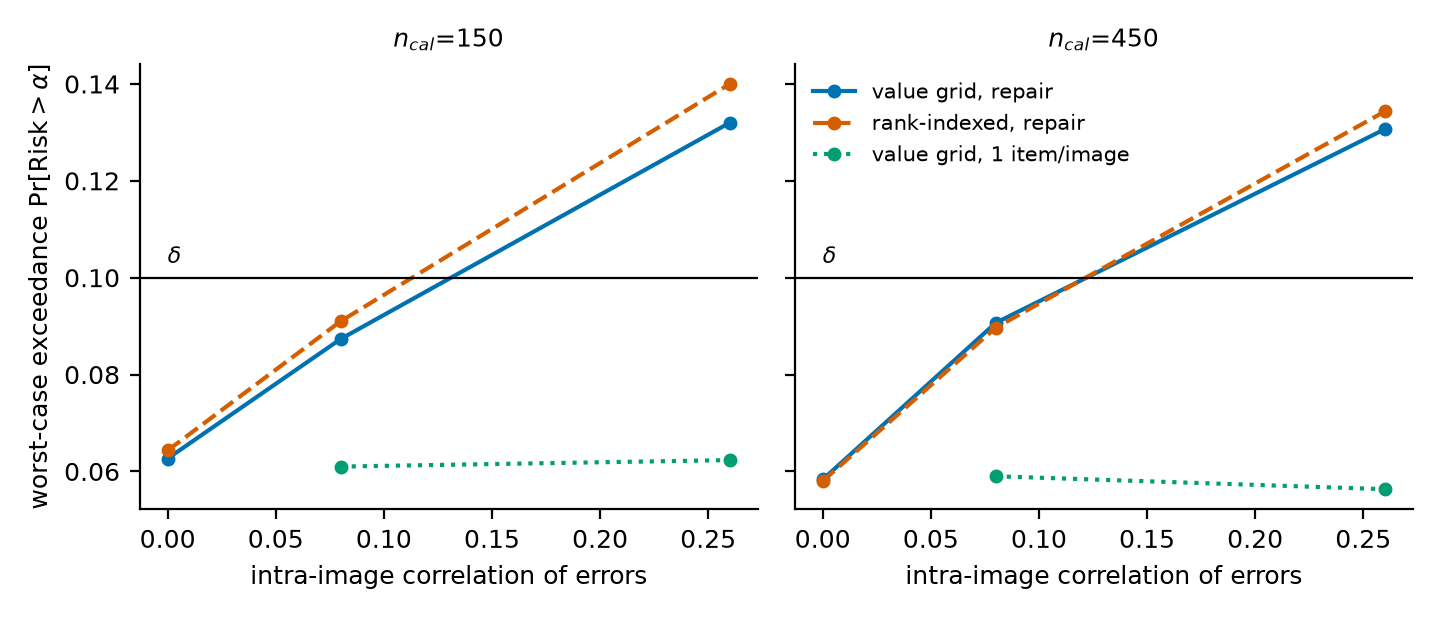
\includegraphics[width=0.95\textwidth]{fig_validity.png}
\caption{Worst-case known-population exceedance over the $\mu$ and $\alpha$ cells, against the intra-image
correlation of errors, with repair. Horizontal line: $\delta=0.10$.}
\label{fig:validity}
\end{figure}

With i.i.d.\ items (ICC $=0$) the exceedance is at most $0.064$ in every cell for both the value-indexed family, which
Theorem~\ref{thm:validity} covers, and the rank-indexed family, which it does not, so the rank-indexed variant is also
conservative here: the missing proof for it is a gap in the argument rather than an observed failure. With positive
within-image correlation the guarantee degrades: at ICC $0.08$ the worst cell is $0.091$, and at ICC $0.26$ the
exceedance of the value-indexed family rises to $0.125$ (filtering) and $0.132$ (repair), above $\delta$, and the rank-indexed
variant to $0.14$. Calibrating on one random item per image restores validity in every cell ($\le0.062$) at the price of a
smaller calibration sample. In the benchmarks used here the measured ICC is slightly negative
(Table~\ref{tab:cohort}), so these data are not in the clustered regime. A benchmark with several correlated questions per image would be, and there the item-level bound
should not be used without the one-item-per-image calibration or a design-effect correction.

\section{Comparison with concurrent methods}
\label{sec:concurrent}

Two methods published in 2026 are close enough to CCRC that a reader will ask what separates them.
Table~\ref{tab:concurrent} compares the three on the dimensions the reviewing literature cares about. The comparison
is conceptual: the benchmarks, backbones and sample sizes differ, so we do not compare numbers across papers and we
did not rerun either method.

\begin{table}[t]
\centering
\caption{CCRC, BCEA \citep{bcea} (version 4, 21 July 2026) and CEBC \citep{mishra2026cebc}.}
\label{tab:concurrent}
\footnotesize
\begin{tabular}{@{}p{0.17\textwidth}p{0.25\textwidth}p{0.25\textwidth}p{0.27\textwidth}@{}}
\toprule
 & CCRC & BCEA & CEBC\\
\midrule
Action on a flagged claim & emit a detector answer, accept, or abstain & acquire more visual evidence, then answer or abstain; the answer is the model's own & rewrite with a VLM, possibly substituting or inserting objects, then delete what remains below threshold\\
Quantity controlled & error rate of the emitted set, accepted and substituted answers together & error rate of emitted claims & per-mention false-accept rate of a detector threshold on hallucinated mentions in base captions\\
Guarantee & finite-sample, probability $1-\delta$ over calibration, i.i.d.\ units & finite-sample, Bonferroni-corrected Clopper--Pearson over a fixed grid; a full-level scan is labelled uncertified & none stated; no theorem, no sampling model\\
Revised output inside the guarantee & yes & not applicable (no revision) & no; the rewrite may use objects at $\tau-0.05$ and is outside the calibration\\
Calibration procedure & fixed-sequence test over values from the fit fold & fixed grid, Bonferroni & one clipped quantile\\
Role of the detector & channel 2: supplies the substituted answer and its margin & optional guide for acquisition & sole arbiter of support\\
\bottomrule
\end{tabular}
\end{table}

\paragraph{BCEA.}
BCEA reduces the abstention floor's practical bite by spending a visual budget to re-read the image and
recalibrating on post-acquisition scores. It stays inside the premise of Proposition~\ref{prop:floor}: acquisition changes how confident the
method is about the model's claim, and which claim is emitted does not change. Its current version certifies a
Bonferroni-corrected Clopper--Pearson test over a threshold grid fixed independently of the calibration sample and
reports certified coverage of $0.23$ without acquisition and $0.32$ with gated acquisition at $\alpha=0.10$; the
coverage figures of $0.28$ and $0.37$ correspond to its uncertified practical variant, which scans the calibration
scores at full confidence. The mechanisms are different (re-scoring a claim versus replacing it) and in principle
composable, since a re-scored claim can still be repaired when the detector is decisive. We have not tested
the composition in this version, and nothing here shows that it helps.

\paragraph{CEBC.}
CEBC is the nearest published method that edits unsupported object mentions in VLM output with an external detector.
Its calibration is a one-sided quantile of detector scores on hallucinated mentions from base captions; its rewrite stage
is not calibrated; and it reports no violation check. Whatever its empirical merit, it is a detector-gated rewriter rather than a certified
selective predictor, and its headline numbers (for example CHAIR$_S$ from $10.0$ to $2.0$) measure a different object
than a certified error rate over emitted claims. CEBC applies to free-form captions and CCRC as evaluated to
yes/no questions; the guarantee of Theorem~\ref{thm:validity} has no free-form counterpart in this paper, and
\S\ref{sec:sequential} gives the reason.

\paragraph{What remains of the novelty claim.}
Among the work we surveyed up to 4 October 2026, CCRC is the one whose certificate covers an emitted answer
that differs from the model's, with the repair gate fixed from fit or external data. CEBC edits without certifying;
BCEA certifies without editing; conformal linguistic calibration \citep{jiang2025clc} certifies a rewritten output
for text-only question answering by generalising claims. The claim is about the combination, in the setting of
object-existence questions, and not about the idea of correcting hallucinations.

\section{Free-form generation: a matched-prefix test of mid-sequence repair}
\label{sec:sequential}

Correction looks more attractive in captions than in yes/no answers: replacing a hallucinated word keeps a
caption that deletion would damage. The extension seems mechanical, and two obstacles are known. Editing a prefix makes
later tokens off-policy, which is feedback covariate shift \citep{fannjiang2022fcs} and falls outside weighted conformal
methods \citep{tibshirani2019}; and per-claim guarantees say nothing about a whole sequence whose length is
data-dependent. Prefix-conditional (Mondrian) $p$-values and e-processes \citep{waudbysmith2024,ramdas2023} could
handle both in principle, leaving the drift of the calibration pool, which on-policy calibration by fixed-point
iteration would address if the correction map were monotone. We measured whether it is before attempting a proof.

\paragraph{Design.}
For each image we generate a caption greedily, locate the first hallucinated object mention at position $t$ using AMBER's
per-image present and absent object lists, and build two prefixes identical up to $t$: one that keeps the hallucinated
word and one that substitutes the best-detected object the image contains. We continue decoding the same number of
tokens from each and count hallucinated mentions in the continuations only. The only difference between the two
continuations is the intervention. The unit is the matched pair ($n=121$ images); there is one repair per pair.

\paragraph{Result.}
In this sample repair makes the continuation worse (Table~\ref{tab:monotone}, Figure~\ref{fig:monotonicity}). Hallucinated mentions
in the continuation rise from $1.207$ to $1.413$, a paired difference of $+0.207\pm0.091$ ($t(120)=2.27$, two-sided
$p=0.025$), with $45$ pairs worsening, $25$ improving and $51$ tied. A Wilcoxon signed-rank test ($p=0.035$) and an exact sign test
($p=0.023$) agree. The Hodges--Lehmann estimate is $0.000$ because $42\%$ of pairs are tied.

\begin{table}[t]
\centering
\caption{Paired matched-prefix test ($n=121$). All $p$-values are two-sided.}
\label{tab:monotone}
\small
\begin{tabular}{lccc}
\toprule
Downstream measure (continuation only) & Original & Repaired & paired difference ($p$)\\
\midrule
Hallucinated mentions (mean)      & 1.207 & 1.413 & $+0.207$ ($0.025$)\\
Hallucinations per $100$ words    & 3.61  & 4.30  & $+0.75$ ($0.011$)\\
Faithful mentions (mean)          & 1.579 & 1.752 & $+0.174$ ($0.077$)\\
Continuation length (words)       & 33.4  & 32.9  & $-0.55$ ($0.092$)\\
Hallucinated share of mentions    & 0.433 & 0.447 & $-0.004$ ($0.884$)\\
\bottomrule
\end{tabular}
\end{table}

\begin{figure}[t]
\centering
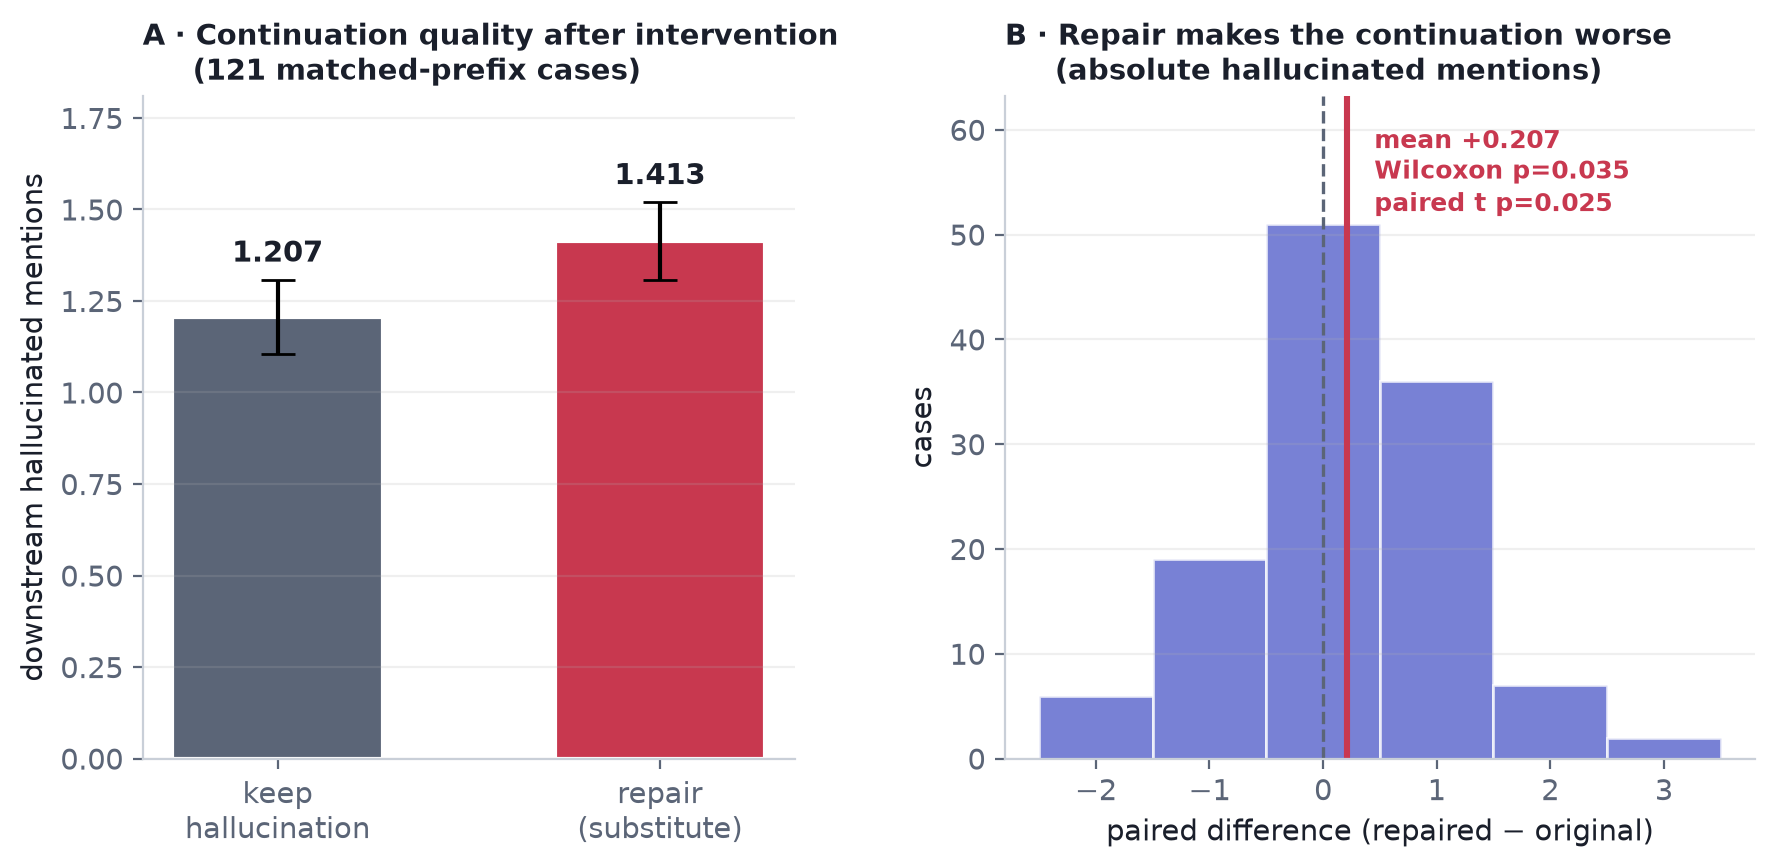
\includegraphics[width=0.9\textwidth]{fig_monotonicity.png}
\caption{(A) Mean hallucinated mentions in the continuation after keeping or repairing the flagged claim (standard errors).
(B) Distribution of the paired difference.}
\label{fig:monotonicity}
\end{figure}

\paragraph{What the experiment can support.}
The result is significant under three tests and under-powered. At the observed paired standard deviation ($0.999$) the
minimum detectable effect at $80\%$ power is $+0.257$, larger than the observed $+0.207$, and about $186$ pairs would be
needed at this effect size. Equivalence testing against a margin of $\pm0.25$ does not establish equivalence
($p=0.317$). The sign is established and the magnitude is not: any value in $[+0.027,+0.386]$ is compatible. The number
of hallucinated mentions rises together with faithful mentions and with mention density; per mention, the hallucinated share does not move
($0.433\to0.447$, $p=0.884$), so the mechanism is denser object talk after repair. A certificate on the count of false
claims is not helped by this, since each additional hallucinated mention counts. The substitution used here is
context-blind, and the finding concerns that rule rather than all correction. What the data withdraw is support
for a monotone correction map and hence for a fixed-point route to a sequential guarantee, at the sample size we have.

\paragraph{A coupling bound.}
For a sequence of claims let $F(O)$ be the number of false claims and $\Risk(O)=\E[F(O)]$ the expected count per
sequence. Let a repair rule replace claims at a random set $P$ of positions, producing $O'$.
Write $W$ for the number of wrong repaired claims, $F_P(O)$ for the number of false \emph{original} claims at the
repaired positions, and $\Delta$ for the signed change in the number of false claims at non-repaired positions
between $O'$ and $O$.

\begin{theorem}[Coupling bound for corrected sequences]
\label{thm:coupling}
$F(O')=F(O)-F_P(O)+W+\Delta$ pointwise, hence
\[
\Risk(O')=\Risk(O)+\E[W]-\E[F_P(O)]+\Iota\ \le\ \Risk(O)+\E[W]+\Iota,\qquad \Iota:=\E[\Delta].
\]
$\Iota$ is signed: a repair that prevents later errors makes it negative. If at most one claim is repaired per
sequence, $\E[W]=\Pr[X\in R]\,\Pr[\text{repair wrong}\mid X\in R]$; in general $\E[W]=\sum_t\Pr[t\in P,\ \text{repair at }t\text{ wrong}]$ is an expected
count over repair opportunities.
\end{theorem}
\begin{proof}
The false claims of $O'$ are those at repaired positions (the wrong repairs, $W$) plus those at non-repaired positions. The false claims of $O$ are
those at repaired positions ($F_P(O)$) plus those at non-repaired positions. Subtracting gives the identity, and taking
expectations gives the equality; $F_P(O)\ge0$ gives the bound.
\end{proof}

In the matched-prefix experiment one claim is repaired per pair, so $\widehat\Iota$ is the paired difference in
the continuation: $+0.207\pm0.091$ additional false claims per repair. That is as large as the direct term for a
repair that is wrong with probability $0.2$, and it cannot be dropped. Certifying $\Risk(O)\le\alpha_1$ and the direct term by
$\alpha_2$ at $\delta/2$ each gives $\Risk(O')\le\alpha_1+\alpha_2+\Iota$ at $1-\delta$, which is useful only
relative to an already-selective base policy, since certifying the uncorrected generation is the object the
abstention floor makes expensive. A sequential procedure would have to price the continuation and not only the claim,
for example by searching over rewrites under an accumulated risk ledger. We leave that open.

\section{Discussion}
\label{sec:discussion}

\paragraph{What the guarantee says.}
With probability $1-\delta$ over the calibration sample, the population risk of the deployed policy, accepted and
substituted answers together, is at most $\alpha$. It says nothing about a single item, about a finite test fold, about
a distribution other than the one the units were drawn from, or about the coverage that results. A sampling model is
part of it: units are i.i.d., and when a benchmark is split at random the iid assumption is a modelling choice about the population
the benchmark represents.

\paragraph{What the evidence supports.}
Under a protocol in which the proved procedure is the evaluated procedure, certified repair gains between $0.8$ and $7.9$ points
of coverage over certified filtering when the gate is fixed on external data; the sign is supported by $65$--$99\%$ of
image-bootstrap datasets and the interval excludes zero on one cell. The statement a reader can rely on is therefore
that the gain is positive in expectation on these benchmarks and small, and that more images would be needed to
size it. Two of the three mechanisms the earlier analysis offered survive in weaker form. Repair does add a few points of coverage; it
does so mostly by confirming answers the model already gave, and corrects almost none of the model's false positives.
The correctness score dominates the coverage, and the start of the fixed sequence dominates the repair on small folds.

\paragraph{Limitations.}
(i) The task is binary object existence, with one detector, three backbones and two benchmark families whose
images overlap; $642$ distinct images are involved in total. (ii) The channel-2 operating point $\theta=0.15$ was fixed
in the extraction scripts and is not varied here; we do not claim it was chosen independently of the benchmarks.
(iii) The external gate for the POPE cells was chosen on AMBER, whose image sources we could not verify to be disjoint from
POPE's COCO images; the guarantee requires the gate to be independent of the calibration sample, and any image overlap
would weaken that independence slightly. (iv) The i.i.d.\ assumption is violated within images when errors are correlated; here the
measured correlation is slightly negative, and \S\ref{sec:validity-audit} shows the guarantee degrades with positive
correlation unless calibration uses one item per image. (v) The bootstrap interval reflects sampling of images from the benchmark, not
of benchmarks from the world. (vi) Free-form generation is not covered and mid-sequence repair worsens the continuation.
(vii) We did not rerun the VLMs, extract signals on additional images, or run BCEA or CEBC.

\paragraph{Next steps.}
The measurement that would most improve the paper is more images: processing the remaining POPE images and a
second detector would narrow the intervals the bootstrap now shows to be wide. A repair rule that
respects the generation context, tested on the free-form setting with the matched-prefix design, is the natural
extension.

\section{Conclusion}
\label{sec:conclusion}

Certified correction replaces an answer the model would have abstained on with a detector's answer and
certifies the emitted set as a whole; the procedure is valid under i.i.d.\ sampling when thresholds and gate are
fixed before calibration. Under a protocol built on that requirement the coverage gain over filtering is small and positive, with an
uncertainty that the available images do not resolve. Most repaired items re-emit the model's answer with detector
confirmation, the model's false positives are not corrected, and the coverage comes mainly from the correctness score.
In generation, mid-sequence repair worsens the continuation. The reproducible pipeline and all negative results are released.


\bibliographystyle{abbrvnat}
\bibliography{refs}

\appendix
\section{Additional results}

\subsection{Audit of all arms}
\label{app:audit}
\begin{table}[h]
\centering
\caption{Certified coverage (\%) with abort rate (ab) and validity statistics for every arm, all items. exc is the
fraction of non-aborted splits whose test-fold risk exceeds $\alpha$; cv is the fraction whose one-sided $90\%$
Clopper--Pearson lower bound on test risk exceeds $\alpha$. The fixed $q{=}0.10$ gate was chosen with knowledge of
these benchmarks and is not certified.}
\label{tab:audit}
\tiny
\resizebox{\textwidth}{!}{\begin{tabular}{lcrrrrrrrrrr}
\toprule
 & & \multicolumn{2}{c}{Filter} & \multicolumn{2}{c}{External gate} & \multicolumn{2}{c}{Fit-fold gate} & \multicolumn{2}{c}{Union ($\delta/3$)} & \multicolumn{2}{c}{Fixed $q{=}0.10$}\\
\cmidrule(lr){3-4}\cmidrule(lr){5-6}\cmidrule(lr){7-8}\cmidrule(lr){9-10}\cmidrule(lr){11-12}
Setting & $\alpha$ & cov.\ (ab) & exc/cv & cov.\ (ab) & exc/cv & cov.\ (ab) & exc/cv & cov.\ (ab) & exc/cv & cov.\ (ab) & exc/cv\\
\midrule
POPE-1500, LLaVA & 0.10 & 68.2 (0) & 0.11 / 0.02 & 77.6 (0) & 0.09 / 0.01 & 77.0 (1) & 0.10 / 0.01 & 72.6 (0) & 0.04 / 0.01 & 71.1 (0) & 0.11 / 0.01\\
 & 0.15 & 85.5 (0) & 0.09 / 0.01 & 92.8 (0) & 0.09 / 0.01 & 92.6 (0) & 0.09 / 0.01 & 89.1 (0) & 0.04 / 0.00 & 87.6 (0) & 0.09 / 0.01\\
\addlinespace
POPE-3000, LLaVA & 0.10 & 76.6 (0) & 0.06 / 0.01 & 83.2 (0) & 0.09 / 0.01 & 82.8 (0) & 0.09 / 0.01 & 79.3 (0) & 0.03 / 0.01 & 78.6 (0) & 0.07 / 0.01\\
 & 0.15 & 90.8 (0) & 0.11 / 0.01 & 95.8 (0) & 0.10 / 0.01 & 95.8 (0) & 0.10 / 0.01 & 94.0 (0) & 0.04 / 0.00 & 92.2 (0) & 0.10 / 0.01\\
\addlinespace
POPE-adv, LLaVA & 0.10 & 44.5 (25) & 0.14 / 0.01 & 37.3 (48) & 0.13 / 0.01 & 41.4 (34) & 0.14 / 0.00 & 28.0 (57) & 0.12 / 0.01 & 48.2 (22) & 0.14 / 0.02\\
 & 0.15 & 72.5 (2) & 0.07 / 0.00 & 82.6 (2) & 0.07 / 0.00 & 82.0 (2) & 0.08 / 0.00 & 72.7 (4) & 0.04 / 0.00 & 76.4 (1) & 0.09 / 0.00\\
\addlinespace
POPE-adv, Qwen2-VL & 0.10 & 76.9 (1) & 0.09 / 0.01 & 69.1 (14) & 0.11 / 0.01 & 71.2 (10) & 0.11 / 0.01 & 68.9 (11) & 0.05 / 0.00 & 79.4 (0) & 0.10 / 0.01\\
 & 0.15 & 94.6 (0) & 0.06 / 0.00 & 95.7 (0) & 0.06 / 0.00 & 95.0 (0) & 0.06 / 0.00 & 92.9 (0) & 0.04 / 0.00 & 95.2 (0) & 0.06 / 0.00\\
\addlinespace
POPE-adv, LLaVA+VCD & 0.10 & 45.8 (14) & 0.14 / 0.01 & 33.5 (46) & 0.23 / 0.04 & 39.6 (30) & 0.21 / 0.03 & 34.2 (37) & 0.10 / 0.01 & 47.8 (11) & 0.14 / 0.01\\
 & 0.15 & 74.4 (0) & 0.11 / 0.02 & 76.8 (0) & 0.11 / 0.02 & 76.1 (0) & 0.11 / 0.02 & 69.4 (0) & 0.04 / 0.01 & 75.7 (0) & 0.11 / 0.02\\
\addlinespace
AMBER(d), LLaVA & 0.10 & 64.4 (0) & 0.10 / 0.01 & 67.5 (0) & 0.09 / 0.01 & 66.8 (1) & 0.10 / 0.01 & 66.4 (0) & 0.06 / 0.01 & 64.4 (5) & 0.09 / 0.02\\
 & 0.15 & 75.7 (0) & 0.12 / 0.02 & 79.6 (0) & 0.13 / 0.01 & 79.5 (0) & 0.13 / 0.02 & 77.7 (0) & 0.06 / 0.01 & 78.8 (0) & 0.13 / 0.02\\
\bottomrule
\end{tabular}
}
\end{table}

\subsection{Protocol ladder and start of the sequence at other targets}
\label{app:ladder}
\begin{table}[h]
\centering
\caption{As Table~\ref{tab:ladder} at $\alpha=0.15$.}
\small
\resizebox{\textwidth}{!}{\begin{tabular}{lcccccc}
\toprule
 & POPE-1500,\ LLaVA & POPE-3000,\ LLaVA & POPE-adv,\ LLaVA & POPE-adv,\ Qwen2-VL & POPE-adv,\ LLaVA+VCD & AMBER(d),\ LLaVA\\
\midrule
conventional protocol (item folds, calibration quantiles, $e_0{=}0$, fixed $q{=}0.10$) & 86.4/88.4 & 91.0/92.4 & 69.3/76.7 & 94.8/95.2 & 75.8/77.2 & 96.2/59.9\\
+ image-grouped folds & 85.8/87.8 & 91.0/92.3 & 70.4/77.7 & 94.5/94.9 & 75.6/76.8 & 95.9/64.7\\
+ fixed value grid and gate (fit fold) & 85.5/87.5 & 90.8/92.2 & 61.8/72.9 & 93.7/94.7 & 63.1/72.4 & 85.1/85.0\\
+ analytic start $e_0{=}1$ & 85.5/87.6 & 90.8/92.2 & 70.9/75.1 & 94.1/94.9 & 73.5/75.1 & 94.2/94.1\\
+ gate chosen on the fit fold & 85.5/92.6 & 90.8/95.8 & 70.9/81.1 & 94.1/94.7 & 73.5/75.5 & 94.2/96.4\\
+ all-item cohort & 85.5/92.6 & 90.8/95.8 & 72.5/82.0 & 94.6/95.0 & 74.4/76.1 & 75.7/79.5\\
\bottomrule
\end{tabular}
}
\end{table}
\begin{table}[h]
\centering
\caption{As Table~\ref{tab:start} at $\alpha=0.05$.}
\scriptsize
\resizebox{\textwidth}{!}{\begin{tabular}{cccrrrrrrrrrrrr}
\toprule
 & & & \multicolumn{2}{c}{POPE-1500,~LLaVA} & \multicolumn{2}{c}{POPE-3000,~LLaVA} & \multicolumn{2}{c}{POPE-adv,~LLaVA} & \multicolumn{2}{c}{POPE-adv,~Qwen2-VL} & \multicolumn{2}{c}{POPE-adv,~LLaVA+VCD} & \multicolumn{2}{c}{AMBER(d),~LLaVA}\\
\cmidrule(lr){4-5}\cmidrule(lr){6-7}\cmidrule(lr){8-9}\cmidrule(lr){10-11}\cmidrule(lr){12-13}\cmidrule(lr){14-15}
$c$ & $e_0$ & $k_{\mathrm{start}}$ & filter & CCRC & filter & CCRC & filter & CCRC & filter & CCRC & filter & CCRC & filter & CCRC\\
\midrule
1.0 & 0 & 45 & 19.6 (35) & 29.2 (18) & 47.0 (2) & 46.9 (9) & 8.6 (80) & 7.9 (82) & 35.4 (17) & 36.7 (19) & 9.8 (74) & 9.6 (75) & 48.0 (0) & 47.2 (5)\\
1.0 & 1 & 77 & 27.5 (14) & 31.4 (16) & 47.2 (1) & 46.9 (10) & 3.2 (94) & 3.2 (94) & 31.6 (46) & 29.6 (50) & 8.7 (82) & 8.7 (82) & 48.2 (0) & 47.8 (6)\\
1.0 & 2 & 105 & 24.2 (32) & 27.2 (30) & 47.8 (0) & 46.4 (10) & 0.5 (99) & 0.5 (99) & 37.1 (40) & 34.3 (46) & 2.2 (96) & 2.2 (96) & 48.3 (0) & 47.7 (6)\\
1.0 & 3 & 132 & 21.2 (50) & 22.2 (51) & 47.8 (0) & 45.5 (12) & 0.0 (100) & 0.0 (100) & 7.4 (90) & 7.3 (90) & 0.3 (100) & 0.3 (100) & 48.2 (0) & 46.3 (9)\\
\addlinespace
1.5 & 0 & 45 & 26.3 (16) & 31.6 (15) & 47.3 (1) & 46.5 (9) & 4.7 (91) & 4.6 (91) & 30.4 (44) & 26.6 (52) & 8.2 (82) & 8.2 (82) & 48.1 (0) & 47.4 (6)\\
1.5 & 1 & 77 & 21.8 (44) & 24.3 (41) & 47.9 (0) & 46.5 (10) & 0.0 (100) & 0.0 (100) & 24.1 (62) & 23.4 (64) & 1.2 (98) & 1.2 (98) & 48.2 (0) & 47.8 (6)\\
1.5 & 2 & 105 & 23.1 (50) & 24.6 (48) & 47.9 (0) & 45.2 (12) & 0.0 (100) & 0.0 (100) & 1.6 (98) & 1.6 (98) & 0.0 (100) & 0.0 (100) & 48.3 (0) & 45.2 (11)\\
1.5 & 3 & 132 & 25.0 (49) & 25.8 (48) & 47.7 (0) & 45.5 (12) & 0.0 (100) & 0.0 (100) & 0.0 (100) & 0.0 (100) & 0.0 (100) & 0.0 (100) & 48.4 (0) & 46.2 (9)\\
\bottomrule
\end{tabular}
}
\end{table}
\begin{table}[h]
\centering
\caption{As Table~\ref{tab:start} at $\alpha=0.15$.}
\scriptsize
\resizebox{\textwidth}{!}{\begin{tabular}{cccrrrrrrrrrrrr}
\toprule
 & & & \multicolumn{2}{c}{POPE-1500,~LLaVA} & \multicolumn{2}{c}{POPE-3000,~LLaVA} & \multicolumn{2}{c}{POPE-adv,~LLaVA} & \multicolumn{2}{c}{POPE-adv,~Qwen2-VL} & \multicolumn{2}{c}{POPE-adv,~LLaVA+VCD} & \multicolumn{2}{c}{AMBER(d),~LLaVA}\\
\cmidrule(lr){4-5}\cmidrule(lr){6-7}\cmidrule(lr){8-9}\cmidrule(lr){10-11}\cmidrule(lr){12-13}\cmidrule(lr){14-15}
$c$ & $e_0$ & $k_{\mathrm{start}}$ & filter & CCRC & filter & CCRC & filter & CCRC & filter & CCRC & filter & CCRC & filter & CCRC\\
\midrule
1.0 & 0 & 15 & 85.5 (0) & 92.6 (0) & 90.8 (0) & 95.8 (0) & 46.1 (36) & 81.9 (1) & 91.9 (3) & 92.6 (2) & 38.9 (47) & 73.4 (4) & 75.7 (0) & 79.5 (0)\\
1.0 & 1 & 25 & 85.5 (0) & 92.6 (0) & 90.8 (0) & 95.8 (0) & 67.6 (8) & 82.9 (0) & 94.3 (0) & 94.9 (0) & 66.2 (11) & 74.7 (2) & 75.7 (0) & 79.5 (0)\\
1.0 & 2 & 34 & 85.6 (0) & 92.6 (0) & 90.8 (0) & 95.8 (0) & 71.4 (3) & 82.4 (1) & 94.3 (0) & 94.8 (0) & 73.2 (2) & 75.2 (1) & 75.7 (0) & 79.5 (0)\\
1.0 & 3 & 43 & 85.6 (0) & 92.6 (0) & 90.8 (0) & 95.8 (0) & 73.2 (1) & 81.3 (2) & 94.5 (0) & 94.9 (0) & 74.4 (0) & 75.6 (0) & 75.7 (0) & 79.5 (0)\\
\addlinespace
1.5 & 0 & 15 & 85.5 (0) & 92.6 (0) & 90.8 (0) & 95.8 (0) & 64.0 (12) & 82.4 (0) & 94.3 (0) & 94.8 (0) & 61.7 (18) & 74.0 (3) & 75.7 (0) & 79.5 (0)\\
1.5 & 1 & 25 & 85.5 (0) & 92.6 (0) & 90.8 (0) & 95.8 (0) & 72.5 (2) & 82.0 (2) & 94.6 (0) & 95.0 (0) & 74.4 (0) & 76.1 (0) & 75.7 (0) & 79.5 (0)\\
1.5 & 2 & 34 & 85.5 (0) & 92.6 (0) & 90.8 (0) & 95.8 (0) & 72.6 (3) & 81.3 (3) & 94.6 (0) & 95.2 (0) & 74.5 (0) & 76.1 (0) & 75.7 (0) & 79.5 (0)\\
1.5 & 3 & 43 & 85.6 (0) & 92.6 (0) & 90.8 (0) & 95.8 (0) & 72.8 (4) & 79.9 (5) & 94.8 (0) & 95.1 (0) & 74.6 (1) & 74.6 (3) & 75.6 (0) & 79.4 (0)\\
\bottomrule
\end{tabular}
}
\end{table}

\subsection{Gain decomposition}
\begin{table}[t]
\centering
\caption{Gain decomposition (points of test coverage), $q=0.10$, all items, conditional on both arms certifying.}
\label{tab:dilution}
\small
\resizebox{\textwidth}{!}{\begin{tabular}{lccccc}
\toprule
Setting & $\alpha$ & threshold moves (\%) & gain & (i) repairs at filter's threshold & (ii) dilution [95\% CI over splits]\\
\midrule
POPE-1500, LLaVA & 0.10 & 31 & 2.79 & 1.89 & 0.89 [0.74, 1.05]\\
 & 0.15 & 25 & 2.06 & 1.43 & 0.63 [0.51, 0.75]\\
\addlinespace
POPE-adv, LLaVA & 0.10 & 24 & 2.75 & 1.94 & 0.81 [0.52, 1.10]\\
 & 0.15 & 26 & 3.04 & 1.59 & 1.46 [0.99, 1.92]\\
\addlinespace
POPE-adv, Qwen2-VL & 0.10 & 18 & 2.17 & 0.93 & 1.24 [0.64, 1.84]\\
 & 0.15 & 3 & 0.37 & 0.31 & 0.06 [0.01, 0.10]\\
\addlinespace
POPE-adv, LLaVA+VCD & 0.10 & 12 & 1.12 & 0.67 & 0.45 [0.25, 0.66]\\
 & 0.15 & 11 & 1.14 & 0.49 & 0.65 [0.28, 1.02]\\
\addlinespace
AMBER(d), LLaVA & 0.10 & 34 & 3.61 & 2.84 & 0.78 [0.33, 1.23]\\
 & 0.15 & 27 & 1.93 & 1.47 & 0.46 [0.20, 0.72]\\
\bottomrule
\end{tabular}
}
\end{table}

\subsection{Multi-start search}
\label{app:multistart}
\begin{table}[h]
\centering
\caption{Certified coverage (\%, abort rate in parentheses) for the single starts $e_0=0$ and $e_0=1$ and for the union over $e_0\in\{0,1,2\}$ at $\delta/3$ each.}
\label{tab:multistart}
\small
\resizebox{\textwidth}{!}{\begin{tabular}{lcccccccc}
\toprule
 & & \multicolumn{3}{c}{filtering} & \multicolumn{3}{c}{CCRC, external gate}\\
\cmidrule(lr){3-5}\cmidrule(lr){6-8}
Setting & $\alpha$ & $e_0{=}0$ & $e_0{=}1$ & multi-start ($\delta/3$) & $e_0{=}0$ & $e_0{=}1$ & multi-start ($\delta/3$)\\
\midrule
POPE-1500, LLaVA & 0.10 & 67.5 (0) & 68.2 (0) & 64.2 (0) & 69.5 (0) & 69.6 (0) & 66.3 (0)\\
 & 0.15 & 85.5 (0) & 85.5 (0) & 83.2 (0) & 92.8 (0) & 92.8 (0) & 91.2 (0)\\
\addlinespace
POPE-3000, LLaVA & 0.10 & 76.5 (0) & 76.6 (0) & 74.4 (0) & 83.2 (0) & 83.2 (0) & 81.2 (0)\\
 & 0.15 & 90.8 (0) & 90.8 (0) & 89.2 (0) & 95.8 (0) & 95.8 (0) & 95.1 (0)\\
\addlinespace
POPE-adv, LLaVA & 0.10 & 36.9 (30) & 44.5 (25) & 31.9 (41) & 39.3 (27) & 46.2 (24) & 33.2 (40)\\
 & 0.15 & 64.0 (12) & 72.5 (2) & 65.1 (3) & 68.2 (8) & 74.4 (1) & 66.5 (2)\\
\addlinespace
POPE-adv, Qwen2-VL & 0.10 & 76.5 (0) & 76.9 (1) & 72.4 (1) & 78.0 (0) & 78.0 (0) & 73.4 (1)\\
 & 0.15 & 94.3 (0) & 94.6 (0) & 91.8 (0) & 95.5 (0) & 95.7 (0) & 92.8 (0)\\
\addlinespace
POPE-adv, LLaVA+VCD & 0.10 & 39.5 (22) & 45.8 (14) & 35.4 (28) & 40.8 (20) & 46.6 (12) & 36.2 (26)\\
 & 0.15 & 61.7 (18) & 74.4 (0) & 64.8 (2) & 76.5 (1) & 76.8 (0) & 66.9 (5)\\
\addlinespace
AMBER(d), LLaVA & 0.10 & 64.4 (0) & 64.4 (0) & 63.4 (0) & 67.5 (0) & 67.5 (0) & 65.4 (2)\\
 & 0.15 & 75.7 (0) & 75.7 (0) & 74.2 (0) & 79.6 (0) & 79.6 (0) & 78.1 (0)\\
\bottomrule
\end{tabular}
}
\end{table}

\subsection{Benchmarks where the detector does not apply}
\begin{table}[h]
\centering
\caption{Filtering (confidence score, image-grouped folds, $400$ splits) where the detector does not apply.
Certified coverage (\%) with abort rate in parentheses.}
\label{tab:sweep}
\small
\resizebox{\textwidth}{!}{\begin{tabular}{lrrrccc}
\toprule
Dataset & images & $\mu$ (\%) & detector value & $\alpha{=}0.10$ & $\alpha{=}0.15$ & $\alpha{=}0.20$\\
\midrule
MME (700) & 350 & 31.1 & 0 & 0.9 (97) & 10.4 (56) & 21.0 (24)\\
GQA testdev (700) & 319 & 27.6 & 0 & 8.5 (72) & 34.6 (18) & 57.7 (4)\\
HallusionBench (447) & 165 & 48.8 & 0 & 0.0 (100) & 0.0 (100) & 0.0 (100)\\
\bottomrule
\end{tabular}
}
\end{table}

\subsection{Grounded-only cohort}
\label{app:grounded}
\begin{table}[h]
\centering
\caption{As Table~\ref{tab:main} restricted to items with a detector value; no bootstrap.}
\small
\resizebox{\textwidth}{!}{\begin{tabular}{lcccccccc}
\toprule
 & & Filter & \multicolumn{2}{c}{External gate} & \multicolumn{2}{c}{Fit-fold gate} & \multicolumn{2}{c}{Fixed $q{=}0.10$}\\
\cmidrule(lr){4-5}\cmidrule(lr){6-7}\cmidrule(lr){8-9}
Setting & $\alpha$ & cov.\ (ab) & cov.\ (ab) & gain & cov.\ (ab) & gain & cov.\ (ab) & gain\\
\midrule
POPE-1500, LLaVA & 0.10 & 68.2 (0) & 77.6 (0) & +9.4 & 77.0 (1) & +8.8 & 71.1 (0) & +2.9\\
 & 0.15 & 85.5 (0) & 92.8 (0) & +7.3 & 92.6 (0) & +7.1 & 87.6 (0) & +2.1\\
\addlinespace
POPE-3000, LLaVA & 0.10 & 76.6 (0) & 83.2 (0) & +6.6 & 82.8 (0) & +6.3 & 78.6 (0) & +2.0\\
 & 0.15 & 90.8 (0) & 95.8 (0) & +5.1 & 95.8 (0) & +5.0 & 92.2 (0) & +1.4\\
\addlinespace
POPE-adv, LLaVA & 0.10 & 43.6 (26) & 36.5 (49) & $-$7.1 & 39.4 (37) & $-$4.2 & 47.4 (22) & +3.8\\
 & 0.15 & 70.9 (2) & 82.2 (1) & +11.3 & 81.1 (1) & +10.2 & 75.1 (1) & +4.2\\
\addlinespace
POPE-adv, Qwen2-VL & 0.10 & 75.6 (1) & 67.7 (16) & $-$7.9 & 68.3 (13) & $-$7.3 & 78.0 (1) & +2.5\\
 & 0.15 & 94.1 (0) & 95.3 (0) & +1.2 & 94.7 (0) & +0.6 & 94.9 (0) & +0.8\\
\addlinespace
POPE-adv, LLaVA+VCD & 0.10 & 45.5 (15) & 32.8 (48) & $-$12.6 & 39.7 (30) & $-$5.8 & 47.6 (12) & +2.1\\
 & 0.15 & 73.5 (2) & 77.2 (1) & +3.7 & 75.5 (2) & +2.0 & 75.1 (1) & +1.6\\
\addlinespace
AMBER(d), LLaVA & 0.10 & 90.9 (0) & 93.6 (0) & +2.7 & 93.3 (0) & +2.4 & 90.1 (2) & $-$0.8\\
 & 0.15 & 94.2 (1) & 96.5 (0) & +2.3 & 96.4 (0) & +2.2 & 94.1 (2) & $-$0.1\\
\bottomrule
\end{tabular}
}
\end{table}

\subsection{Reproducibility}
All numbers in the paper are generated from per-item signals by the scripts in the released repository
(\texttt{conformal\_followup/revision}): \texttt{attach\_image\_ids.py} recovers and verifies image identifiers;
\texttt{ccrc\_rev.py} implements the protocol; \texttt{regress\_legacy.py} checks that the conventional-protocol mode reproduces the
numbers of the baseline implementation; \texttt{exp\_*.py} produce the results files and \texttt{make\_tables.py},
\texttt{make\_figures.py} the tables and figures. Splits are deterministic in the seed.

\end{document}
